\documentclass[a4paper]{report}

%====================== PACKAGES ======================

\usepackage[english]{babel}
\usepackage[utf8x]{inputenc}
%pour gérer les positionnement d'images
\usepackage{float}
\usepackage{amsmath}
\usepackage{amssymb}
\usepackage{algorithm}
\usepackage{algorithmic}
\usepackage{graphicx}
\usepackage{pdfpages}
\usepackage[colorinlistoftodos]{todonotes}
\usepackage{url}
%pour les informations sur un document compilé en PDF et les liens externes / internes
\usepackage{hyperref}
%pour la mise en page des tableaux
\usepackage{array}
\usepackage{tabularx}
%pour utiliser \floatbarrier
%\usepackage{placeins}
%\usepackage{floatrow}
%espacement entre les lignes
\usepackage{setspace}
%modifier la mise en page de l'abstract
\usepackage{abstract}
%police et mise en page (marges) du document
\usepackage[T1]{fontenc}
\usepackage[top=2cm, bottom=2cm, left=2cm, right=2cm]{geometry}
%Pour les galerie d'images
\usepackage{subfig}
%Pour les codes sources
\usepackage{listings}
\renewcommand{\algorithmicrequire}{\textbf{Input:}}	%Use Input in the format of Algorithm
\renewcommand{\algorithmicensure}{\textbf{Output:}}	%Use Output in the format of Algorithm
%====================== INFORMATION ET REGLES ======================

%rajouter les numérotation pour les \paragraphe et \subparagraphe
\setcounter{secnumdepth}{4}
\setcounter{tocdepth}{4}

\hypersetup{							% Information sur le document
pdfauthor = {Simon CHANU},			% Auteurs
pdftitle = {Shepherd Report},			% Titre du document
pdfsubject = {},		% Sujet
%pdfkeywords = {Tag1, Tag2, Tag3, ...},	% Mots-clefs
pdfstartview={FitH}}					% ajuste la page à la largueur de l'écran
%pdfcreator = {MikTeX},% Logiciel qui a crée le document
%pdfproducer = {}} % Société avec produit le logiciel

%======================== DEBUT DU DOCUMENT ========================

\begin{document}

%régler l'espacement entre les lignes
\newcommand{\HRule}{\rule{\linewidth}{0.5mm}}

%page de garde
\begin{titlepage}
    \title{ \normalsize \textsc{Project Report} 
    		\\ [0.5cm]
            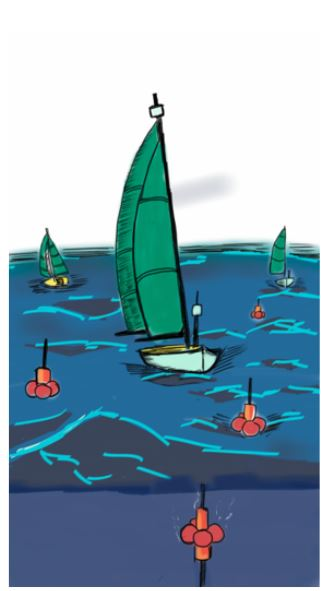
\includegraphics[scale=0.6]{image/logo_SHEPHERD.JPG} % Ou autre image
            \\ [0.3cm]
            \HRule{} 
            \\ [0.5cm]
            \LARGE \textbf{\uppercase{SHEPHERD Project}} 
            \\ [0.20cm]
            \HRule{} 
            \\ [1.0cm]
            
\includegraphics[scale=0.6]{image/logo_ENSTA.jpg}
            %\\
            %\textsc{\textbf{ENSTA Bretagne}}
            \\ [0.5cm]
            \normalsize \today \vspace*{0\baselineskip}
    }

    \date{}
    
    \author{
            \textbf{Students}\\
            \textsc{El Jawad.A,  Chanu.S, Sola.Y, Welte.A, Soulie.C, Benet.P, Mehdi.N, } \\
            \textsc{Galland.A, Barronier.R, El Abdalaoui.Z, Finand.C, Zhu.L, Pertierre.S, } \\
            \textsc{Ennouhi.F, Bernardes.E, Tanguy.F, Martin.P} \\
            \\
            \textbf{Supervisor}\\
            \textsc{Luc Jaulin, ENSTA Bretagne} 
    }

    \maketitle
\end{titlepage}

%page blanche
%\newpage
~
%ne pas numéroter cette page
\thispagestyle{empty}
\newpage

% Abstract
\begin{abstract}

	\footnote{Author : Simon CHANU} The SHEPHERD Project aims to command a swarm of robotic oceanographic buoys by the astute use of the different directions of the current at along the water column, with the help of an acoustic localization system provided by robotic sailboats acting as shepherds. This paper describes the simulation created to validate the foundations of the project. This simulation uses simple models and equations to effectively command a swarm of robots.

\end{abstract}

\tableofcontents
%ne pas numéroter le sommaire

\newpage

\listoffigures
\thispagestyle{empty}
\setcounter{page}{0}

\newpage

%espacement entre les lignes d'un tableau
\renewcommand{\arraystretch}{1.5}

%====================== INCLUSION DES PARTIES ======================

~
\thispagestyle{empty}
%recommencer la numérotation des pages à "1"
\setcounter{page}{0}
\newpage

\chapter{Presentation of the Shepherd project}
\section{Given issue}
\footnote{Section Written by Camille Finand}
The issue the project is trying to solve in an issue raised by IFREMER. They wish to realize a three dimensional map of the turbulent flow of currents in ocean. To this end, they wish to deploy a swarm of buoy robots, left to drift with the current, at a know variable depth.

Our mission was to design such a swarm of buoy robots, their shepherd sailing boats\footnote{see "Our solution" section for more details} and to realize a simulation of experiment through interval calculus.


\section{Our solution}

\footnote{Section Written by Camille Finand}
In order to solve the given issue we decided to introduce "shepherd sailboats".
Because our buoys  are unable to locate themselves via GPS while under water, the sailboats act as interfaces between the GPS network and the underwater buoys.

There will be four shepherd boats providing a frame for the buoys to locate themselves in.
This localization will be realized through calculating the \emph{Time Difference Of Arrival} \footnote{see section 1.3 TDOA method} of four acoustics pings.
Each boat send a unique synchronized ping received by all the buoys that can then estimate their position relatively to the boats.

This allows us to have a relative control over our swarm of buoys dispersion.
Having a map, or at least a local map, we can indeed chose the current that best match our expectations for the chosen dispersion or displacement of the swarm.
Such a dispersion and or position will be a fixed chosen interval of positions in the four sailboats frame.

However the positioning is relative to the sailboats and not necessarily known by the buoys. So they need to come back to the surface during the mission in order to precisely update their position and centralize their data.
\begin{figure}[H]
  \centering
  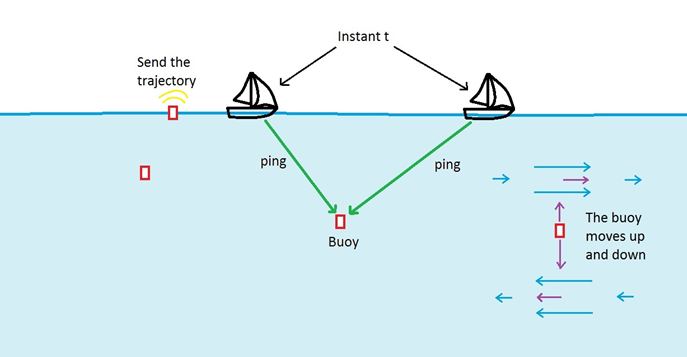
\includegraphics[scale = 0.9]{image/ProjectSchem.png}
  \label{ProjectSchem}
  \caption{Buoy localization and control}
\end{figure}

The Buoys are controlled in depth via Ballasts and pressure captors. The sailboats are not controlled in position but rather follow lines that forms triangle. It is indeed much simpler than having them strictly sticking to a point, and we don't really need them to be on a specific place at a given time, they just need to be close enough and far enough to each other to give the buoys an adapted frame in which to position themselves.

% 
\section{Interval Analysis}
\subsection{Introduction}
\footnote{Section written by M. Fadil Ennouhi and F. Tanguy} 
Interval analysis aims to use sets of intervals, rather than
sets of real numbers in arithmetic. 
Thus performing the same simple operations such as sum and multiplication on intervals. The usefulness of this particular method lies in its tolerance to uncertainty. In the SHEPHERD Project our sensors and methods inherently cause uncertainty, making the use of Interval Analysis in the localization procedure almost compulsory.

\subsection{Application}
In our simulation we restricted the problem to a buoy trying to find its location using the data fed by four sailboats. We then use the SIVIA algorithm to estimate the position of the buoy. 
The Set Inversion Via Interval Analysis globally consists of performing set inversion. 

\begin{equation}
	\text{if f: } \mathbf{R^n} \rightarrow \mathbf{R}^m \text{ and } \mathbf{Y} \subset \mathbf{R^m}
\end{equation}

\begin{equation}
	\mathbf{X}=\{x \in \mathbf{R^n}\ | f(x) \in \mathbf{Y} \}=f^-1\mathbf{(Y)} \nonumber\\
	\label{eq: Set Inversion}
\end{equation}

We strongly recommend viewing the videos of M. Luc Jaulin on this subject which can be found on YouTube.

\begin{figure}[H]
	\centering
	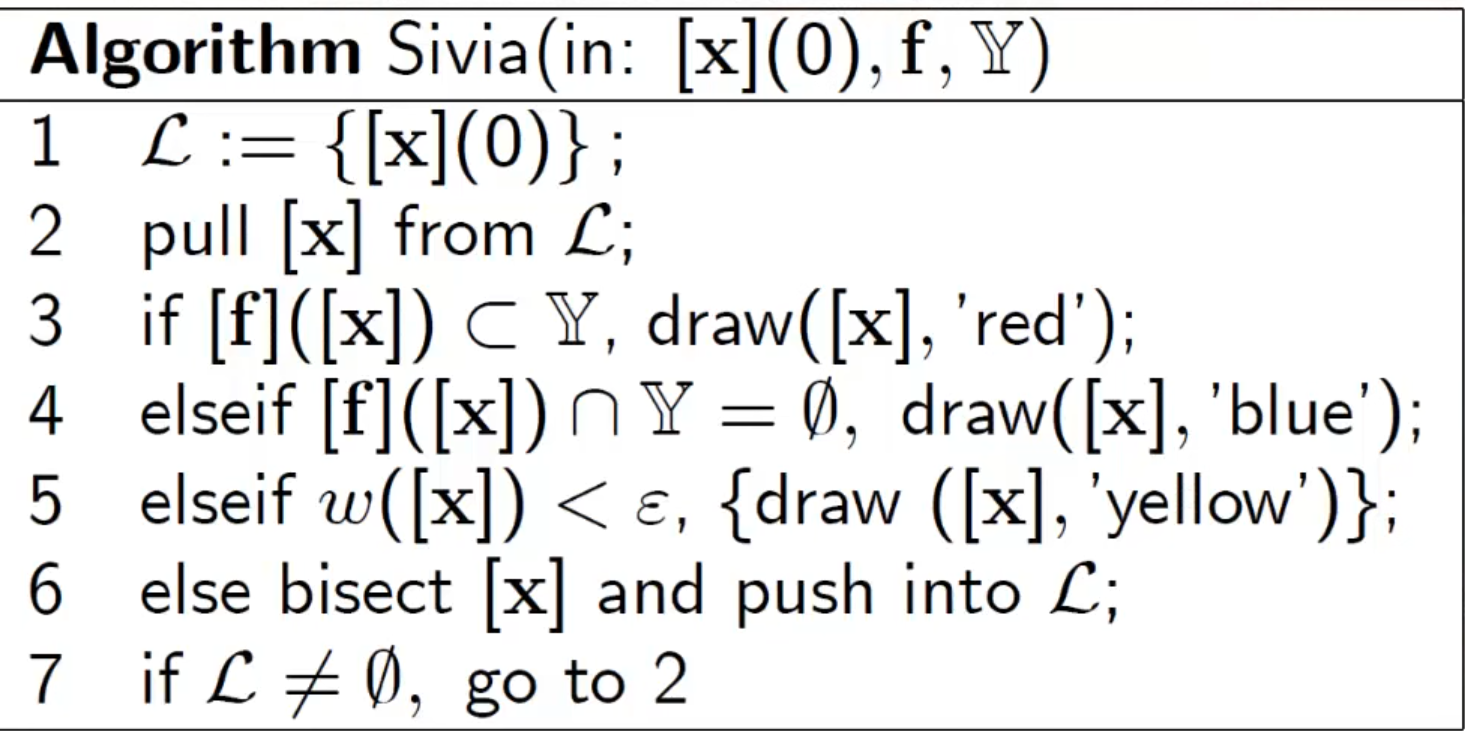
\includegraphics[width=0.4\linewidth]{image/sivia.png}
	\caption{The SIVIA algorithm.}
	\label{fig:SIVIA}
\end{figure}

With the SIVIA algorithm, a list of boxes is generated which corresponds to the localization of the robot. There are three different areas, one representing the position of the robot (the inner area). The outer area does not contain the robot, and the last area correspond to the border, the size of this area depends on the minimum size of the boxes.
\begin{figure}[H]
	\centering
    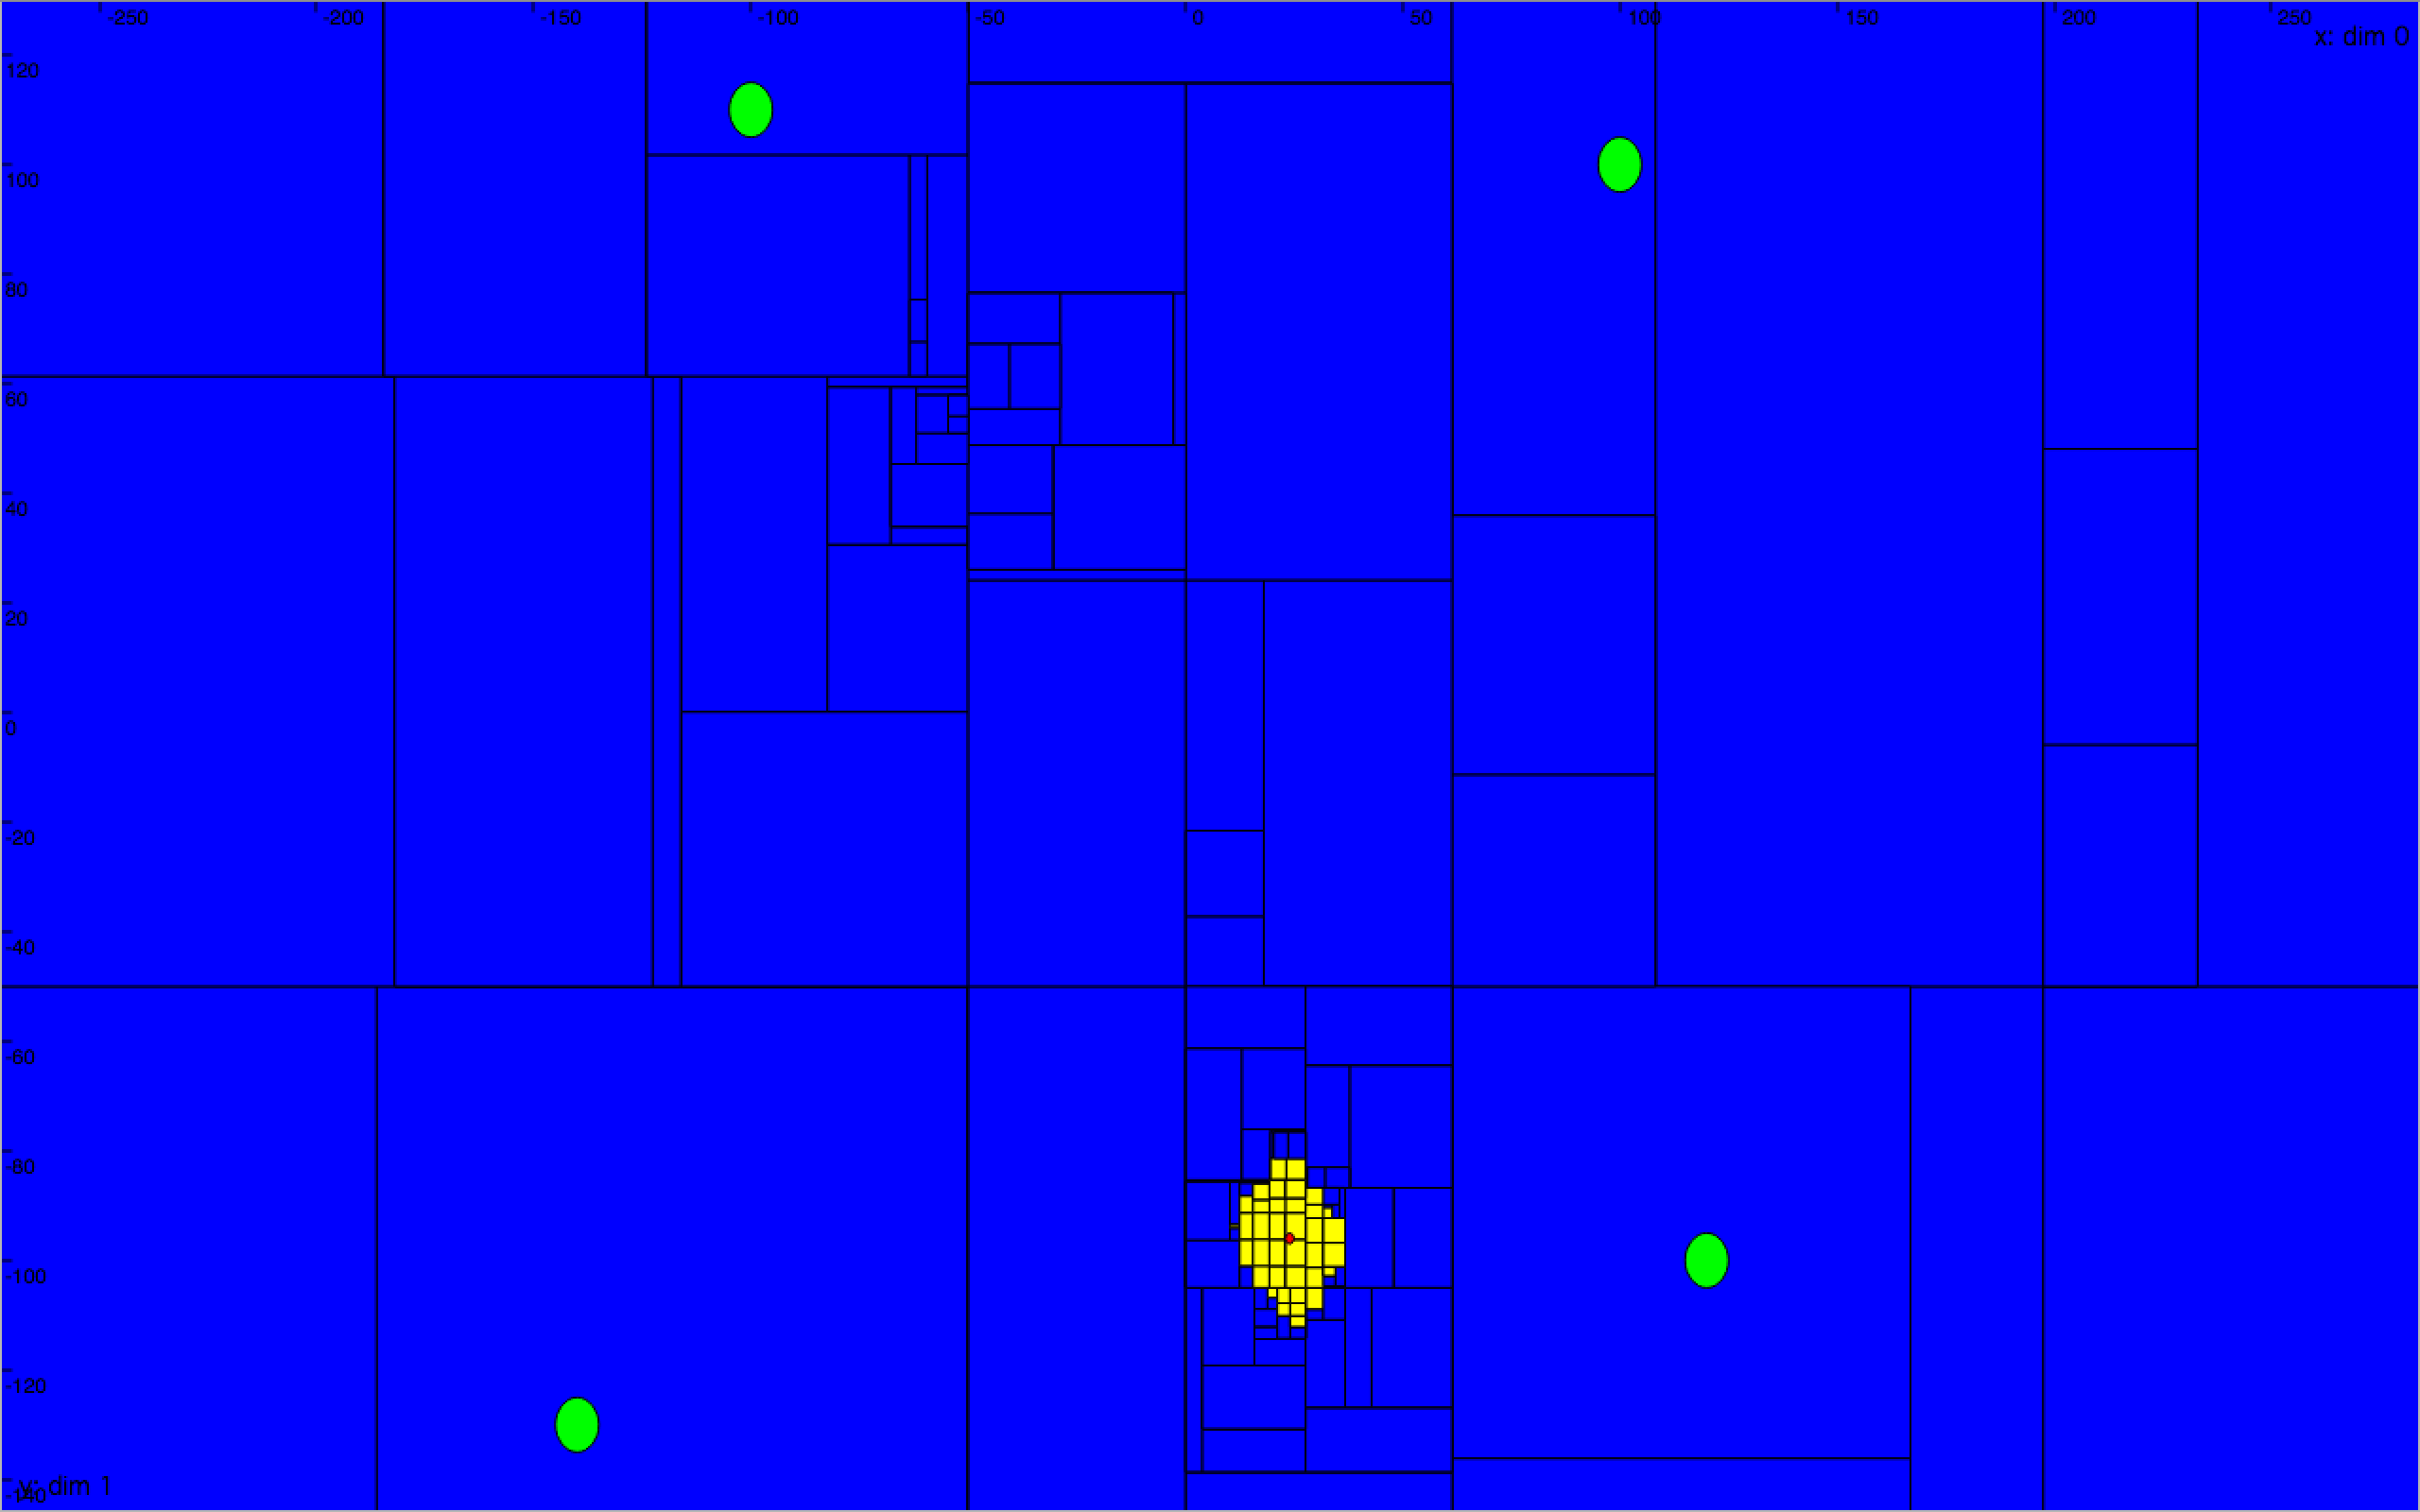
\includegraphics[width=0.4\linewidth]{image/loca_IA.png}
    \begin{center}\caption{ Illustration of the SIVIA algorithm (blue:outer area, red:inner area(buoy), yellow:estimated position of the buoy green: sailboats)}\end{center}
    \label{fig:SIVIA picture}
\end{figure}

\section{TDOA} \label{section:tdoa}
\subsection{Introduction}
\footnote{Section written by E. Bernardes and S. Pertierre} 
In our settings we have four boats that should simultaneously send signals to the buoy, informing their positions (known due to each boat's GPS system) and time of emission (each boat has also an internal clock, considered to be synchronized). 
%
The buoys have to be programmed in a way that make it possible for them to receive these data and calculate their position. 

One possible way to solve this problem is to put a clock inside each buoy.
%
In this way, using the fact that we know the signal's velocity in the sea, we can easily calculate the distances of the buoy to each one of the boats by doing the following calculation:

\begin{equation}
	d_n = ||p - q_n|| = c(t_n - t_0)
	\label{eq:distance}
\end{equation}

Where $d_n$ is the distance of the buoy to the $n$th boat, $q_n = (q_{nx},q_{ny},q_{nz})$ is the position of said boat, $p = (p_x,p_y,p_z)$ is the buoy's position in the sea, $c$ is the signal's velocity in the medium, $t_0$ is the time of emission and $t_n$ is the time when the buoy receive the $n$th boat's signal. 
%
We can calculate all distances in this way and then triangulate the buoy's position.

It is indeed a simple and efficient method of calculation. Nevertheless, it can be difficult to guarantee that the buoy's internal clock is well synchronized with those of the boats, raising the possibility of high uncertainties in the calculations.
%
It is not impossible to do so, but the needed precision clock can be expensive. The Time Difference of Arrival (TDOA) method is proposed to replace this method of calculation and overcome this difficulty.

\subsection{Method principle}
The method consists in substituting the buoy's clock with a chronometer.
%
The chronometer is not capable of knowing the exact moments of the signals arrivals, but it is able to keep track of the time difference between each signal.

When the buoy receives the first boat's signal, if launches the chronometer and waits for the arrival of the other signals, keeping track of the time between then.
%
They buoy stores then the values $\tau_2 = t_2 - t_1$, $\tau_3 = t_3 - t_1$ and $\tau_4 = t_4 - t_1$; as shown in the Figure \ref{fig:time_differences}.
%
\begin{figure}[H]
	\centering
	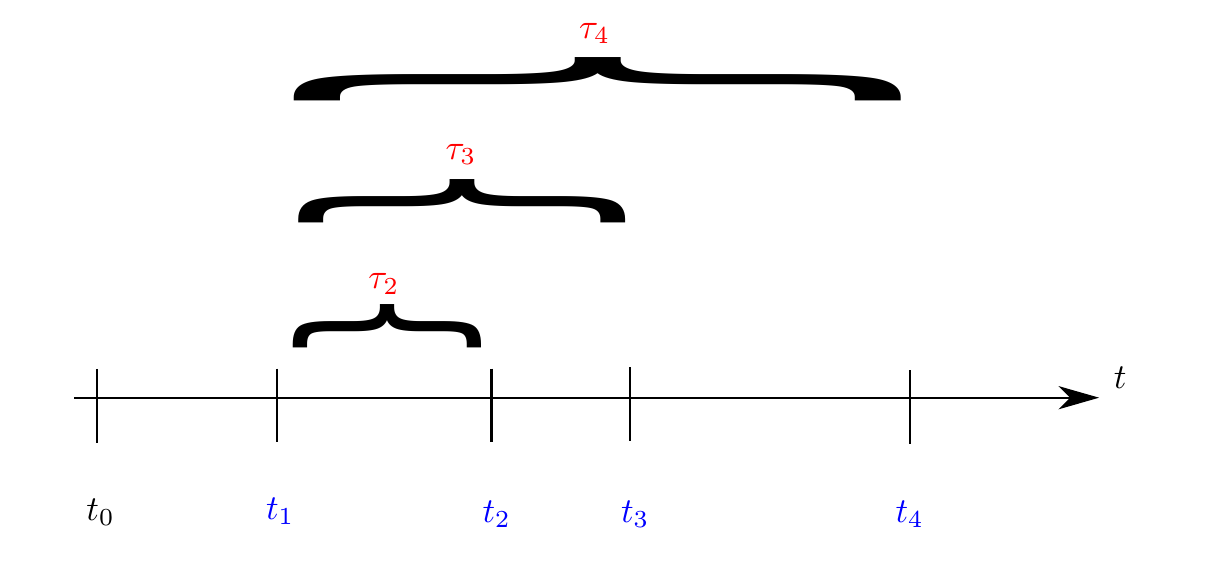
\includegraphics[width=0.7\linewidth]{image/time.png}
	\caption{Time difference values are stored by the buoy.}
	\label{fig:time_differences}
\end{figure}
%
The equation \ref{eq:distance} is still valid, and applying it to our project, we have the system of linear equations described in \ref{eq:distance_system}.
\begin{align}
d_1 = ||p - q_1|| &= c(t_1 - t_0) \nonumber \\
d_2 = ||p - q_2|| &= c(t_2 - t_0) \\
d_3 = ||p - q_3|| &= c(t_3 - t_0) \nonumber \\
d_4 = ||p - q_4|| &= c(t_4 - t_0) \nonumber 
\label{eq:distance_system}
\end{align}
%
Substituting the time differences $\tau_n$ in \ref{eq:distance_system}, we have the following final system:
\begin{align}
||p - q_1|| &= c(t_1 - t_0) \nonumber \\
||p - q_2|| &= c(t_1 + \tau_2 - t_0) \\
||p - q_3|| &= c(t_1 + \tau_3 - t_0) \nonumber \\
||p - q_4|| &= c(t_1 + \tau_4 - t_0) \nonumber 
\label{eq:distance_tdoa}
\end{align}
Since $q_n$, $c$, $t_0$ and $\tau_n$ are all known, then the only unknowns in the system are $t_1$, $p_x$, $p_y$ and $p_z$. Since we have 4 equations and 4 unknowns, we can easily solve this system to find the $p$ vector.
%
Since the buoy's are also equipped with ballasts, we also known the value $p_z$ in our case, our number of equations is bigger than our number of unknown variables.

\subsection{Geolocation problem with random error}
\footnote{The subsection "1.4.3 Geolocation problem with random error" were written by Lei Zhu.}
We assume we are in 2D and there are 4 sailboat (as described in our problem definition). We generate a gaussian random variable $\epsilon_i$ with mean  0 and variance $e_i$. We not the time arrival of source 1 signal $t_1$, it may contain the receiver clock offset.\\
We have thereby 4 equations: 
\begin{align}
||p - q_1|| &= c(t_1 - t_0) + \epsilon_0\nonumber \\
||p - q_2|| &= c(t_1 + \tau_2 - t_0) + \epsilon_1\\
||p - q_3|| &= c(t_1 + \tau_3 - t_0) + \epsilon_2\nonumber \\
||p - q_4|| &= c(t_1 + \tau_4 - t_0) + \epsilon_3\nonumber\\
\label{eq:distance_tdoa_}
\end{align}

Known variables are: $c$, $t_0$, $q_i$, $\tau_i$.

Unknown variables are: $p$, $t_1$,$\epsilon_i$

The problem is undetermined because of the noise on the estimation of distances.

The Geolocation problem becomes the following minimization problem:

\begin{equation}
J(\mathbf{x}, t_1) = \sum \Big ( ||\mathbf{x-x_1}|| - c(\tau_i+t_1-t_0) \Big )^2 / e_i^2 ,\tau_0=0
\end{equation}


\chapter{Team management methods}
\section{Scrum}

\footnote{The section "2.1 Scrum" and its subsections "2.1.1 Agile Software Development" and "2.1.2 Scrum Methodology" were written by Yoann SOLA.}

\subsection{Agile Software Development}


The traditional methods of project management, such as the "V-Model" for example, are not appropriate with software engineering. Indeed, they are too inflexible, they induce a lack of reactivity and they ask for too many deliverables. These methods are predictive methods because they need to plan every single detail of the project, before even starting to code anything.\\

A proof of this inefficiency is the "Chaos Report", published in 1995 by the Standish Group, which studied about 8380 software projects, taken from 365 companies. It showed that 16,2\% of the projects were compliant with the initial forecasts, 52,7\% of them were over the initial budget and went over the initial deadline, and 31,1\% of them were cancelled during their development.\\

Based on this observation, 17 experts in software engineering decided to create in 2001 the Agile Alliance and "The Manifesto for Agile Software Development", which describes the values of the Agile methodology in software engineering. There are four fundamental values in the Agile methodology :
\begin{itemize}
  \item people and communication BEFORE processes and tools
  \item operational features BEFORE the documentation
  \item interacting with the client INSTEAD OF contractual relations
  \item accepting the change INSTEAD OF always following initial plans\\
\end{itemize}

Here are some of the most known methods : ASD (Adaptative Software Development), Crystal, DSDM (Dynamic Software Development Method), Lean, Scrum, XP (eXtreme Programming). We used the Scrum methodology in the SHEPHERD Project.\\

\subsection{Scrum Methodology}

The principle of the Scrum methodology is to organize the project in phases called "sprints" (see Figure \ref{fig:scrum_overview}).\\ 

\begin{figure}[H]
	\centering
	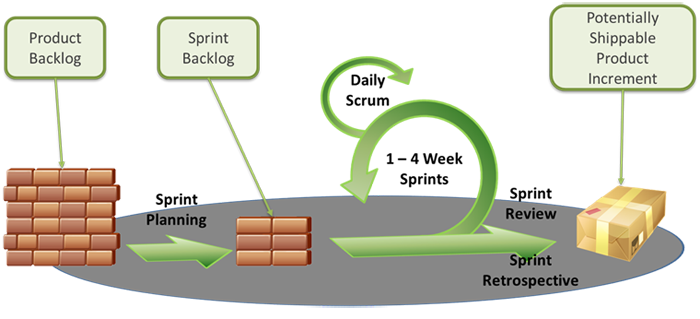
\includegraphics[width=0.7\linewidth]{image/SCRUM-overview-resize.png}
	\caption{An overview of the Scrum methodology.}
	\label{fig:scrum_overview}
\end{figure}

\vspace{1cm}
Indeed, each time a feature of the software is defined by the team (at the beginning or during the project), it is added to a database called the "Product Backlog". \\

A sprint is often a phase of several weeks, which has to produce a fully operational prototype at its end, even if the prototype includes a feature which is not going to be kept for the final version of the software. For that purpose, the features that are going to be implemented during the current sprint are taken from the Product Backlog and are stored in an other database called the "Sprint Backlog".\\

In order to be sure that no one is encountering some troubles, daily morning meeting of 15 minutes are organized by the team, called "Scrums".\\

Moreover, the Scrum methodology uses some useful tools such as the "Kanban Board" (see Figure \ref{fig:kanban}) and the "Burn-down Chart" (see Figure \ref{fig:burndown_chart}), which allows to check if the work will be finished on time if we kept the current pace of work.\\

\vspace{1cm}

\begin{figure}[H]
	\centering
	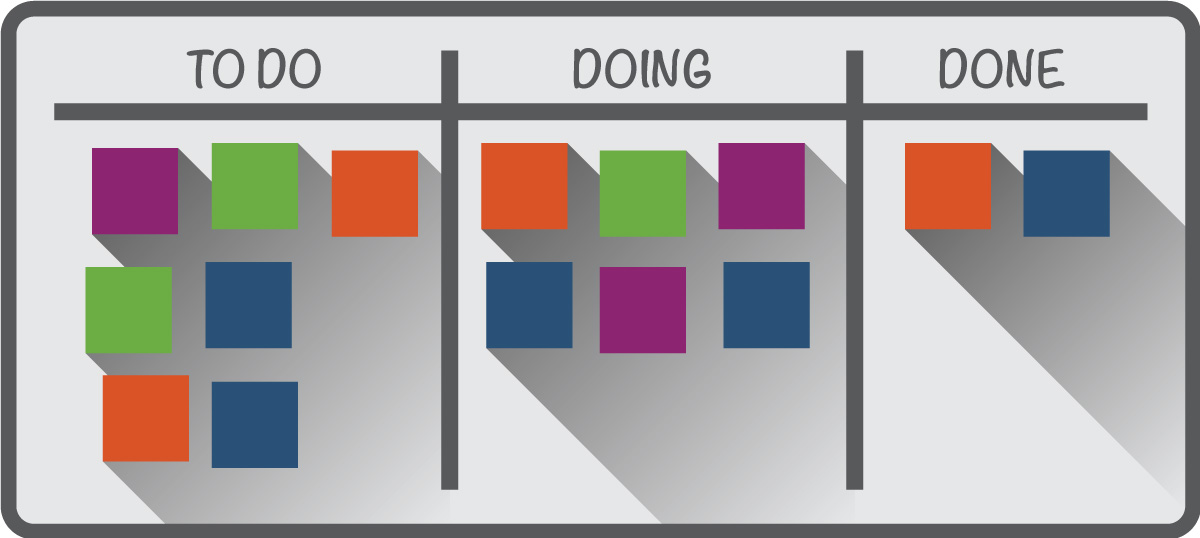
\includegraphics[width=0.7\linewidth]{image/kanban-1.jpg}
	\caption{An example of a kanban Board.}
	\label{fig:kanban}
\end{figure}

\begin{figure}[H]
	\centering
	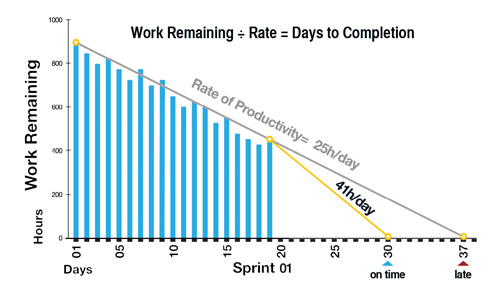
\includegraphics[width=0.7\linewidth]{image/burndown-chart-formula.jpg}
	\caption{An example of a burn-down chart.}
	\label{fig:burndown_chart}
\end{figure}

Finally, three roles are defined by the Scrum methodology for each member of the team :

\begin{itemize}
	\item the Product Owner : it is the person who has to be constantly in relation with the client and has to fill the Product Backlog with him.
	\item the Scrum Master : this is the project manager who has to apply correctly the Scrum methodology and has to be sure that each member of the team has good working conditions.
	\item member of the Scrum Team : this is the team of developer which has to implement features from the Product Backlog.\\
\end{itemize}

In order to implement the Scrum methodology in the SHEPERD project, we use an online platform that allows to easily manage all aspects of this Agile software development method : taiga.io (see Figure \ref{fig:taiga_logo}).

\begin{figure}[H]
	\centering
	
\includegraphics[width=0.6\linewidth]{image/taiga_io.png}
	\caption{Logo of the platform taiga.io.}
	\label{fig:taiga_logo}
\end{figure}

\section{Github}
\footnote{Section written by Simon Chanu}

Github is a website created as free public code repository that facilitate the use of the version control system named Git.

\subsection{Introduction to Git and Version control systems}
\subsubsection{Version control system}
A version control system is a powerful tool used by software development teams to increase the efficiency of coding in team. It is heavily used, if not essential to nowadays software development. It can be a standalone application (such as Git) or it can be embedded in other applications or webapplications (such as Wikipedia). There is a large number of different software that provides a version control system (VCS), but the most commonly used nowadays is Git.\\
\\
The VCS several advantages : 
\begin{itemize}
	\item \textbf{Simultaneous coding} : two members of a team can edit the same file then merge theirs modifications. Thus it allows for efficient teamwork. There is no need anymore to warn the other people of the team that you are working on this specific file and the others must not modify it. This is by far the most interesting feature by making merging code very easy.
    \item \textbf{Versioning} : there is no need to create lots of backup anymore. You can revert the code to previous modifications.
    \item \textbf{Branching} : the code can be separated in different versions. This tool can be used to store versions of the code for different OS for example. But a more common use today is to split versions to implement a new but still buggy feature in the code while the ancient version stays the same. This system will be explained with git in details later.
    \item \textbf{Cloud developpement} : The code can be stored locally or on a remote server. Therefore this is decentralized : it allows to get the sourcecode from anywhere you want and work on it very easily. Moreover if the developer makes a huge mistake and delete everything, he can just download it back to his computer from the remote server. 
\end{itemize}

\subsubsection{Git}

Git is a version control software created by Linus Thorvald (Creator of Linux) in 2005. It was created at the begining as a development tool for the linux kernel. The tool much quicker, secure and supporting distributed development that any version control development at that time, 
This software is available on Linux, Windows, Mac, Solaris. \footnote{https://git-scm.com/downloads} \\

\begin{figure}[H]
	\centering
	
\includegraphics[width=0.2\linewidth]{image/git.png}
	\caption{Logo of Git}
	\label{fig:git_logo}
\end{figure}

Git is now the most widely used source code management tool with 42.9\% of professional software developers using it.

\footnote{https://eclipse.org/org/community\_survey/Survey\_Final\_Results\_2012.xls}

\subsubsection{How does it work ?}

In this section, we will focus on the practical use of Git. First of all, git is a command line software. The main commands are explained below. 
\\
\paragraph{Commands} 
\begin{itemize}
	\item \textbf{git clone} : clone a repository from a remote server to a local folder.
    \item \textbf{git status} : give the current status of the repository and the state of its files. It gives informations about the changes in the repository : which file has been modified, deleted, created, which modification will be sent to the remote in case of a commit push. 
    
    \item \textbf{git pull} : the main command to recover the changes from the remote server. If some changes have been made to your local copy of the code, it will warn you an try an automatic merge of the files. If there is conflicts that can't be resolved automatically, it will warn the user and let it take care of them. It advised to commit any changes to your local copy before pulling from the remote. 
    
    \item \textbf{git add} : validate the changes so can be inserted in a commit. 
    
    \item \textbf{git commit} : register the changes of the local repository so they can be sent to the remote. A git commit must have an explanatory message which describes the changes and why did they happened. This message can be short or long but an input is required from the user. A good habit is to always make comprehensive messages about the changes, so if there is any problem, the code can be easily reverted to a previous commit.
    
    \item \textbf{git push} : the main command to send the local changes to the remote. It sends the commit you have registered with git commit. If any changes has been made on the remote and they haven't been pulled, then the push will be rejected. The user must pull the changes or merge the codes to be able to push all the commits. 
    
    \item \textbf{git merge} : merge two version of a repository together. It takes one version and merge inside the code from the other version. If the merge can't be done automatically because of unresolvable conflicts, a merging process will begin. With a git status it is possible to see the conflicting files. When the conflicting files have been modified, add them and commit them to resolve the merge.   
    
\end{itemize}

\paragraph{Branches}

As it was said above, the code can be split into different existing version among the same repository. These version are called branches. The figure \ref{fig:gitbranch_logo} explains how to use it effectively. 

In a professional software project there is at least usually two branches : \textit{Master} and \textit{develop}. 
\begin{itemize}
	\item \textbf{Master} is the stable, reliable last working version of the code. It's the one customers will download.
    \item \textbf{develop} is the unstable, but as stable as possible, development branch. This is the next iteration of the software. Any developed features end up in the \textit{develop} branch, waiting to be extensively tested before it is allowed to move into the \textit{master} branch
    \item \textbf{Features branches} are usually the rest of the branches. They are created when an independent feature of the software is developed. The development can continue in the branch until finished. Then it can be merged into \textit{develop} for further testing.
\end{itemize}

\begin{figure}[H]
	\centering
	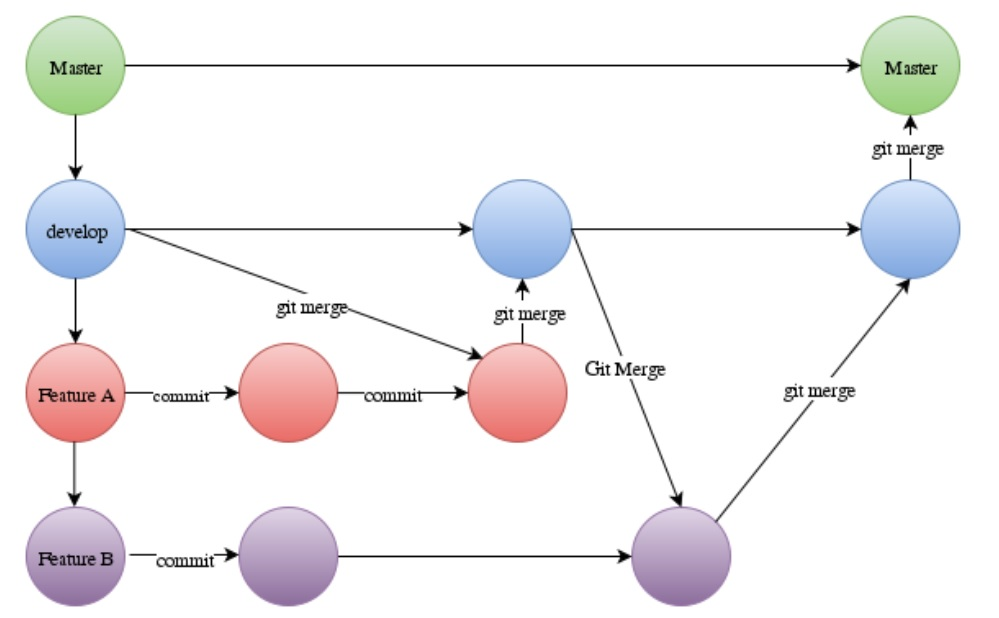
\includegraphics[width=1\linewidth]{image/GitBranch.jpg}
	\caption{Branching system}
	\label{fig:gitbranch_logo}
\end{figure}

This system simplify greatly the workflow. Each merge from develop into master is a new release. Each new feature has it's own branch. On the figure \ref{fig:gitbranch_logo}, it's possible to see this workflow : 
\begin{enumerate}
	\item A new improvement for the software is planned with several features (A and B). The \textit{develop} branch is already up to date with the \textit{master} branch.
    \item The branches from the features are created. They both comes from \textit{develop}.
    \item Some developers work on the features and add, commit then push some changes.
    \item At some point, the dev team from \textit{Feature A} has finished their job. In order to always have the latest version, they merge the code from develop into their branch, resolve the conflicts on their branch, and debug the software. Then they merge automatically into \textit{develop} from \textit{Feature A}
    \item The team of \textit{Feature B} does the same job after.
    \item Then when the software is fully debugged and tested. The \textit{develop} branch can merge into \textit{master}. This is a release. 
\end{enumerate}

You can find more about how to work collaboratively with git \href{https://www.atlassian.com/git/tutorials/comparing-workflows}{here}. If you want to find tutorials about git, it's \href{https://openclassrooms.com/courses/gerez-vos-codes-source-avec-git}{here}.

\subsection{Github}

\begin{figure}[H]
	\centering
	
\includegraphics[width=0.4\linewidth]{image/github.jpg}
	\caption{Logo of Github}
	\label{fig:github_logo}
\end{figure}

Github is a website created in 2008 by Tom Preston-Werner, Chris Wanstrath and PJ Hyett. It provides an internet hosting service and an web based git and project manager. This website provides free remote servers to host the repositories. This access is public and anyone can see the source code pushed on on Github unless a subscription is paid.\\
\\
This website provides as well project management tools, such as a kanban board, a way to specify an track issues on the code, and a interface for most of the difficult git operations. The use of these services are free and require only an inscription.\\
\\
Our project being an open-source research project. The ease of use and the tools provided made this website the best candidate to host our remote repositories. Therefore we decided to create an organization on the website to host our repositories. \\
\\
This organization can be found at \href{https://github.com/ENSTA-Bretagne-Shepherd}{https://github.com/ENSTA-Bretagne-Shepherd}

\subsection{Architecture of the project} 

\subsubsection{First decentralized architecture}

At first we decided to decentralize our work into 3 repositories : Shepherd-Simulation, Shepherd-Display, Shepherd-Localization. Then these projects would be included as submodules into Shepherd-Main. Another repository, called Ressources-internes-et-administration has been created to host our work documents on the software.\\
\\
It happened that this first approach was not very effective. Indeed several types of display have been developed and the number of repository has been multiplied. Moreover the communication between the different parts of the code was difficult to implement.

\subsubsection{Migration on ROS}

That's why a Shepherd-Ros-Structure repository has been created. We integrated the code from the other repository inside ROS. ROS is a middleware that will be presented later in the report. With this integration the project needs only one repository. As presented above, we follow the good rules of conduct in the use of git. Our master branch is the stable up-to-date version of the code and the develop is the development one.

\chapter{Simulation theory} \label{section:simulation}
\section{Simulation of the environment}

\footnote{The section "3.1 Simulation of the environment" was written by Lei Zhu.}

Taking the complexity of modeling a lac into consideration, we had made some simplifications to our simulated environment. \\

The situation of wind in the real world is really intricate. Even the most experienced meteorologist cannot predict the variation of wind for a 100\% accuracy. In our case, it is next to impossible to simulate the wind in an open sea area. Even if we generate randomly the force, this makes no sense except give out a confusing motion of the sailboat under irregular wind. Conversely, if we suppose the wind as constant, we don't really lost the similarity to real word. Meanwhile, we get a lot of time saved as well as the illustration simplified.\\

For the part of waves, we studied the existing work by Mr.Ponte about the analytical solutions of plausible oceanic flows.The mathematic model of multiple 3D eddies is given as Equation \ref{eq:eddies}. \\
\begin{equation}
\begin{aligned}
\psi&= \sum \psi_i e^{-||\mathbf{x-x_i}||^2/R_i^2} \times \cos \frac{N}{c_n}(z+h)  \\
c_n &=\frac{NH}{n\pi} \space ( n>0 \space  , \space \frac{N}{c_0}=0 )  \\
u &=-\partial_y \psi = \sum \psi_i \frac{2y(y-y_i)}{R_i^2} e^{-||\mathbf{x-x_i}||^2/R_i^2}   \\
v &=\partial_x \psi = \sum \psi_i \frac{-2x(x-x_i)}{R_i^2} e^{-||\mathbf{x-x_i}||^2/R_i^2} 
\label{eq:eddies}
\end{aligned}
\end{equation}\\

This model and simulation of eddies enlightened us. However, we find that the sailboat will always work on the sea level and we do not need a 3D simulation of the water. Furthermore, from this model we take notice of that the water stream on the sea level is rather small than under the water. Therefore we chose to ignore the wave so that waves are not simulated eventually.\\

In brief, our simulated environment is under a series of assumption:
\begin{itemize}
\item There is no wave on the horizontal surface;
\item The water stream is negligible;
\item The wind is with unchangeable power and direction.
\end{itemize}


\section{Simulation of the sailboats}
\footnote{The section "3.2 Simulation of the sailboats" was written by Lei Zhu.}
\subsection{External forces and assumption}

As explained in the previous chapter, we analyzed the complexity and compared the result of different choices, and finally we assume that the wind is constant and the water surface is static.\\

Chiefly, there are two media, air and water, are in touch with the sailboats directly. Among all the forces given by air and the water, the friction and damping are insignificant. For this reason, there are also only two kinds of external forces can give out perceptible influence on our simulative sailboats: the wind and the wave. There is no force from the land. \\

To sum up, we designed our method for simulating the the wind and the wave: the wave is supposed to be zero and the wind is a constant force with a fixed direction.

\subsection{State representation}

\begin{figure}[H]
	\centering
	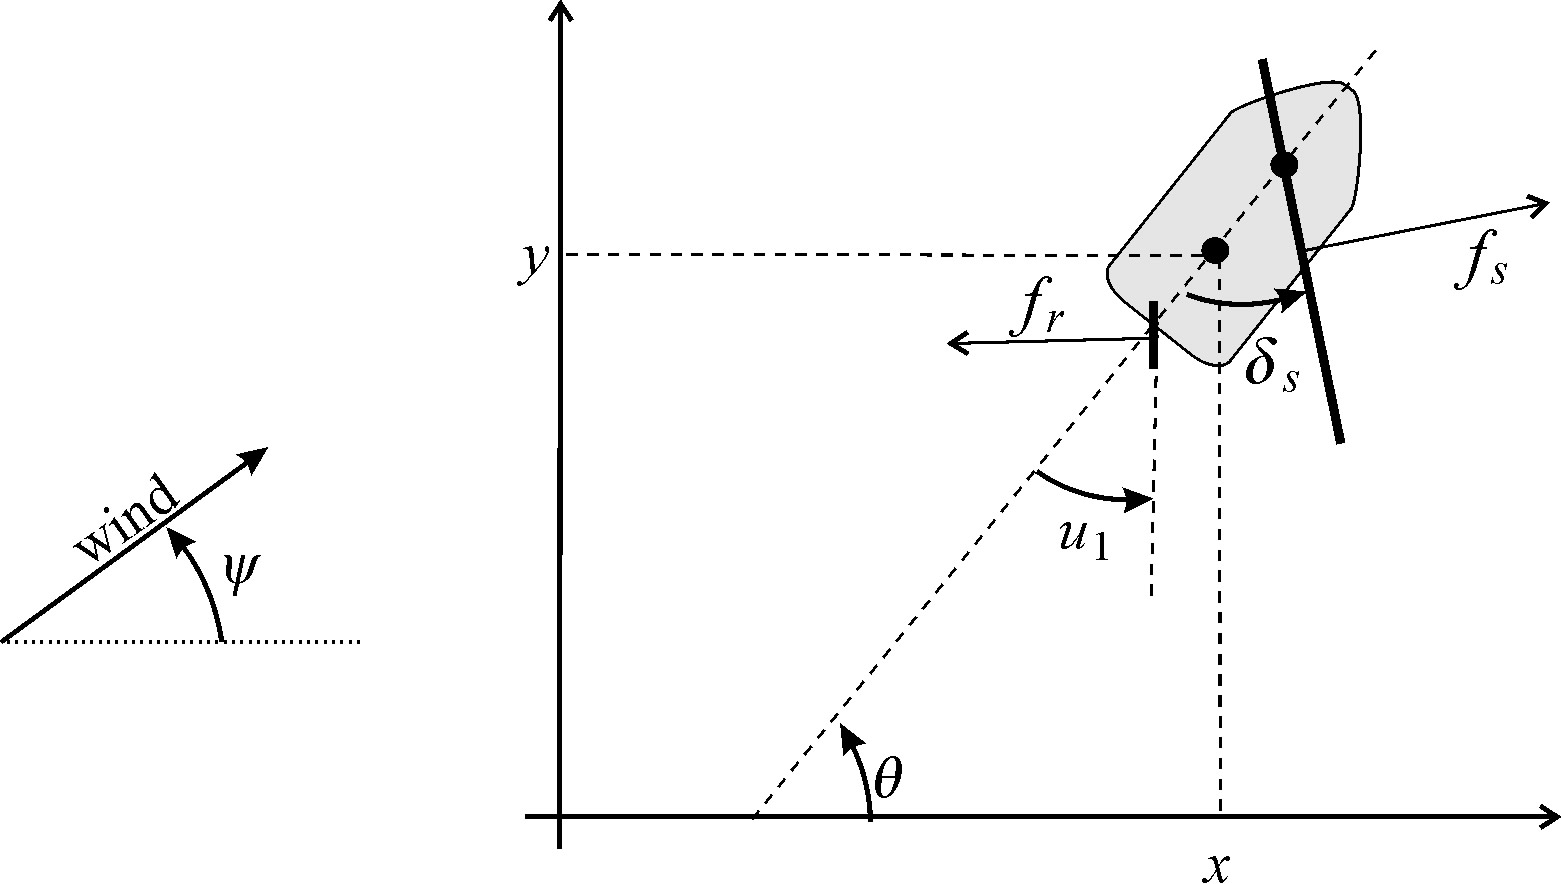
\includegraphics[width=0.6\linewidth]{image/state_representation.jpg}
	\caption{Force illustration and state representation of sailboat}
	\label{fig:state_repre}
\end{figure}



As shown in Figure \ref{fig:state_repre}, we denote a triple $(x, y, \theta)$ to represent the state of the boat. Here x and y is its geometry coordinate while $\theta$ is its heading. Except for the 3 state variables, all the others are used for calculation. Their physic meaning and units are shown in Table \ref{tab:used_var}.

\begin{table}[ht]
\centering
\caption{\label{tab:used_var}Used variables in sailboat state representation.}
\begin{tabular}{c|l|c}
\hline\hline
Variable & Physic Representation & Unit \\
\hline\hline
%\midrule
$v$ & advancing speed & m/s\\
$\omega$ & angular speed & rad/s \\
$\psi$ & wind angle &  rad \\
$f_s$ & force of the wind & N \\
$f_r$ & force of the water on the rudder & N \\
$\delta_s$ & sail angle & rad \\
$\delta_r$ & rudder angle (input) &  rad \\
$\delta_s^{max}$ & maximum angle of the sail(input) & rad\\

\hline\hline
\end{tabular}
\end{table}


\subsection{Control algorithm}

Given 2 points $\mathbf{a}$ and $\mathbf{b}$ to pass through, a sailboat can be controlled by a model-free method \cite{robmob}. As we have mentioned in previous subsection, the sailboat has two inputs which are the rudder angle $u_1 = \delta_r$ and the maximum angle of the sail $u_2 =\delta_s^{max}$. We realized a controller by Algorithm \ref{alg_sailboat_controller}, witch was proposed my Mr.Jaulin on his paper \cite{jaulin2013interval}.\\

\begin{algorithm}

\centering
\caption{Sailboat controller algorithm}
\label{alg_sailboat_controller}
\begin{algorithmic}[1] %此处的[1]控制一下算法中的每句前面都有标号 
\REQUIRE $\mathbf{m}$,$\theta$, $\psi$, $\mathbf{a}$, $\mathbf{b}$, $q$
\ENSURE $\delta_r$,$\delta_s^{max}$, $q$
\STATE $e=det(\frac{\mathbf{b}-\mathbf{a}}{||\mathbf{b}-\mathbf{a}||},\mathbf{m}-\mathbf{a})$
\IF{$|e|>r$}
	\STATE $q=sign(e)$ \\
\ENDIF
\STATE $\phi=angle(\mathbf{b}-\mathbf{a})$\\
\STATE $\bar{\theta}=\phi-atan(\frac{e}{r})$\\
\IF{$cos(\phi-\bar{\theta})+cos\zeta<0 $ or $(|e|<r $ and $(cos(\psi-\phi)+cos\zeta<0))$}
	\STATE $\bar{\theta}=\pi+\psi-q\zeta$ \\
\ENDIF
\STATE $\delta_r=\frac{\delta_s^{max}}{\pi}sawtooth(\theta-\bar{\theta})$\\
\STATE $\delta_s^{max}=\frac{\pi}{2}(\frac{cos(\psi-\bar{\theta})+1}{2})^\frac{log(\frac{\pi}{2\beta})}{log(2)}$\\

\end{algorithmic} 
\end{algorithm}

This algorithm stands for the control of a sailboat with 3 sensors. That is to say, the heading $\theta$, the wind angle $\psi$ and the position of its physic center $\mathbf{m}=(x,y)$ can be captured all the time during its advance process. For the part of actors, $u_1$ and $u_2$ are the two motors to control the movement of sailboat. Therefore, the controller will give out $u_1$ and $u_2$ as output.\\

In this algorithm, we used a very simple idea: when the error between the aim and reality surpass a threshold, the aim will be adjusted by a coefficient. Then with the help of two functions atan() and sawtooth, it is not complicated to generate a feedback.\\

More concretely, we designed a triangle path of side 100m for each sailboat. And 4 sailboats will work together to follow their triangles respectively.


\section{Simulation of the buoys}
\subsection{The Controller of the buoys}

\footnote{The subsection "3.3.1 Controller of the buoys" was written by Yoann SOLA.}

By default, buoys constantly go up and down inside a water column of the ocean, in order to measure the direction of ocean currents at different depths. They can go down until a depth of 1 km and their speed cannot be over 1 m/s. They are able to move vertically thanks to ballasts.\\

They are able to know the direction of ocean currents at a given level of depth by measuring their own acceleration. Indeed, the acceleration of the buoy has the same direction than the direction of ocean currents. This is due to the fact that buoys are moved by ocean currents.\\

In order to prevent buoys from drifting too far, they need to move towards the barycenter formed by the 4 sailboats. This principle allows to keep the group cohesion between buoys.\\

As buoys know the ocean currents of a given water column, they can reach the depth (thanks to their ballasts) which is going to correspond to the best ocean current allowing to move towards the barycenter of the sailboats.\\

Finally, they must surface every 5 hours in order to synchronize their internal clock with GPS signals.





\subsection{The state equations of the buoys}

\footnote{The subsection "3.3.1 Controller of the buoys" was written by Alexandre GALLAND.}

We consider that our system, the sea, can be represented by an incompressible fluid. Thus, we can define a stream function noted $\psi$, which will determine the map of displacement of a particle in the fluid.
Futhermore, we consider that the buoy will behave as a passive particle, letting itself drift with the current.
In the case of two-dimensional, divergence-free Eulerian velocity fields, the equations of motion for a passive particles are : \begin{equation}
\left\{\begin{matrix}
\frac{\mathrm{d} x}{\mathrm{d} t}= u(x,y,t)=\frac{\partial \psi }{\partial y}\\ 
\frac{\mathrm{d} y}{\mathrm{d} t}= v(x,y,t)=-\frac{\partial \psi }{\partial x}
\end{matrix}\right.
\end{equation}

where \textbf{u(x)} = [u(x,y,t),v(x,y,t)].
We will consider the following system as the equations describing the dynamics of advected impurities
\begin{equation}
\left\{\begin{matrix}
\frac{\mathrm{d^2} x}{\mathrm{d} t^2}= \delta \frac{\mathrm{D} u}{\mathrm{D} t} -\mu (\frac{\mathrm{d} x }{\mathrm{d} t}-u)\\ 
\frac{\mathrm{d^2} y}{\mathrm{d} t^2}= \delta \frac{\mathrm{D} v}{\mathrm{D} t} -\mu (\frac{\mathrm{d} y}{\mathrm{d} t}-v)
\end{matrix}\right.
\end{equation}

where 
$
\frac{\mathrm{D} \mathbf{u}}{\mathrm{D} t} = \frac{\partial \mathbf{u} }{\partial t}+\mathbf{(u. \nabla )u}
$,
$\delta = \frac{\rho_f}{\rho_b}$
is the ratio of the fluid density $\rho_f$ to the density of the buoy $\rho_b$, and
$\mu \simeq 1$ is the dynamic viscosity ofthe water.
$\delta \frac{\mathrm{D} \mathbf{u}}{\mathrm{D} t}$ represents the force per unit volume that would be exerted by the fluid on a fluid particle placed at the position of the impurity (similarly to the Archimede's principle).The second terms represents the Stockes drag felt by the buoy whose velocity is different from the flow velocity.\\

This equation does not yet consider the dsiplacement induced by the ballasts.The ballast can be compared as a syringe filled with water, connected to the extern environment. A piston pushes (or pulls) water ouside (or inside) the buoy, changing its volumic mass.
The command received by the simulation from the controller is understood by the simulation as the desired speed for the piston in the ballast.
The vertical acceleration of the buoy is then computed using Newton's second law.\\
\begin{equation}
\frac{\mathrm{d^2} z}{\mathrm{d} t^2}= g-\rho_w \frac {\left ( V-\xi S \right )}{m}
\end{equation}
where $m$ is the mass of the buoy, $V$ its volume when the ballast is empty, $S$ the surface of the piston, and $\xi$ the place of the piston in the ballast (if $\xi = 0$ the ballast is empty). $\rho_w$ is the volumic mass of the water, and $g$ is the gravitation acceleration.\\
The final form of the dynamic equation is then 
\begin{equation}
\left\{\begin{matrix}
\frac{\mathrm{d^2} x}{\mathrm{d} t^2}= \delta \frac{\mathrm{D} u}{\mathrm{D} t} -\mu (\frac{\mathrm{d} x }{\mathrm{d} t}-u)\\ 
\frac{\mathrm{d^2} y}{\mathrm{d} t^2}= \delta \frac{\mathrm{D} v}{\mathrm{D} t} -\mu (\frac{\mathrm{d} y}{\mathrm{d} t}-v)\\
\frac{\mathrm{d^2} z}{\mathrm{d} t^2}= g-\rho_w \frac {\left ( V-\xi S \right )}{m}
\end{matrix}\right.
\end{equation}
\\

In our simulation, we tried out two different two-dimensional stream equation :
\begin{equation}
\psi = A*cos(a_x x+a_y y)
\end{equation}
where $A=2$, and $a_x = a_y = 1$
\begin{equation}
\psi = \sum \psi _i \frac{\left \| \mathbf{X}-\mathbf{X_i} \right \|^2 }{R_i ^2}e^{ -\frac{\left \| \mathbf{X}-\mathbf{X_i} \right \|^2 }{R_i ^2}}
\end{equation}
The first equation creates for small values of A,$a_x$ ,$a_y$ what looks like a chaotic behavior for the buoys.The associated current is a series of vortex close to each other.\\

The second equation is the equation of a stream composed of a multiple water whirl indexed by i. $\mathbf{X_i}$ is the center of the water whirl i, $\psi _i$ represents the rotation speed of the whirl, and $R_i$ represents its range of effect. This representation match correctly the observations of the ocean stream close to the surface. \\

The simulation will cumpute the dispacement of the buoys using the Euler method. The main drawback of using Euler, is the fact that we have to know the exact duration between every iterations. If it is not the case, after a certain period of time, the positions of the buoys might vary from the reality. However, ROS is able to calculate precisely these durations, making the simulation closer to the reality. 




\chapter{Simulation architecture}
\section{ROS presentation}
\footnote{This Section was written by Romain Baronnier}

ROS (Robot Operating System) is the most commonly used middleware in robotic application. The suite was first released in 2007 by Willow Garage, a robotics research lab in California.\\
\begin{center}

\includegraphics[scale=0.4]{image/ros.png}
\end{center}

The Middleware are computer software that allow us to develop new program in a modular fashion. It work as an interface between the different block of our programs. It allows programmer to begin writing their code with a basis.The block Architecture facilitate the flow between simulation and reality : changing the simulation block by real data from real sensor doesn't necessitate to change the whole code. Middleware are frequently used in Simulation, Network system and Robotics.\\

ROS works with a Node architecture, our different blocks become Node in a web of shared Data. Every shared information are Topic that can be broadcasted by Ros's publisher and any node can subscribe to receive update on those informations.Those subscriber can launch Callback function when they receive new data, giving us the possibility to apply traitement to those data. Ros Node can be written in a lot of programming language but the two most commonly used are Python and C++. Moreover as the programs are not directly interfaced but use ROS, we can write some nodes in python and some in C++ and make them communicate without any compatibility problem. We exploited this feature as some of our developper prefer Python while some choose C++.\\

\renewcommand{\lstlistingname}{Code}
\begin{lstlisting}[language=C++, caption={Simple Publisher}, frame=single]
#include "ros/ros.h"
#include "std_msgs/String.h"
#include <sstream>
int main(int argc, char **argv)
{
  ros::init(argc, argv, "talker");
  /**
   * NodeHandle is the main access point to communications with the ROS system.
   * The first NodeHandle constructed will fully initialize this node, and the last
   * NodeHandle destructed will close down the node.
   */
  ros::NodeHandle n;
  /**
   * The advertise() function is how you tell ROS that you want to
   * publish on a given topic name.
   */
  ros::Publisher chatter_pub = n.advertise<std_msgs::String>("chatter", 1000);
  ros::Rate loop_rate(10);
  int count = 0;
  while (ros::ok())
  {
    /**
     * This is a message object. You stuff it with data, and then publish it.
     */
    std_msgs::String msg;
    std::stringstream ss;
    ss << "hello world " << count;
    msg.data = ss.str();
    ROS_INFO("%s", msg.data.c_str());
    /**
     * The publish() function is how you send messages. The parameter
     * is the message object. The type of this object must agree with the type
     * given as a template parameter to the advertise<>() call, as was done
     * in the constructor above.
     */
    chatter_pub.publish(msg);
    ros::spinOnce();
    loop_rate.sleep();
    ++count;
  }
  return 0;
}
\end{lstlisting}

\renewcommand{\lstlistingname}{Code}
\begin{lstlisting}[language=C++, caption={Simple Subscriber}, frame=single]
#include "ros/ros.h"
#include "std_msgs/String.h"

void chatterCallback(const std_msgs::String::ConstPtr& msg)
{
  ROS_INFO("I heard: [%s]", msg->data.c_str());
}

int main(int argc, char **argv)
{
  /*You must call one of the versions of ros::init() before using any other
   * part of the ROS system.
   */
  ros::init(argc, argv, "listener");

  /* NodeHandle is the main access point to communications with the ROS system.
   * The first NodeHandle constructed will fully initialize this node, and the last
   * NodeHandle destructed will close down the node.
   */
  ros::NodeHandle n;
  /* The subscribe() call is how you tell ROS that you want to receive messages
   * on a given topic.
   */
  ros::Subscriber sub = n.subscribe("chatter", 1000, chatterCallback);

  /* ros::spin() will enter a loop, pumping callbacks.  With this version, all
   * callbacks will be called from within this thread (the main one).  ros::spin()
   * will exit when Ctrl-C is pressed, or the node is shutdown by the master.
   */
  ros::spin();

  return 0;
}
\end{lstlisting}
\section{ROS architecture of the project}
	\footnote{written by Alaa El Jawad and Sergio Pertierre}  
ROS provides lots of infrastructure, tools and capabilities as it was explained in the previous section. It means that there are so many differents ways to do the same task. So, in this section we will explain using diagrams how ROS was implemented for project SHEPHERD, demonstrating the advantages of using this middleware.

Basically, there are the diagram which shows the general view of the project and then two diagrams presenting the detailed architecture of sailboats and buoys.
\subsection{Overview of the architecture}
The diagram below shows the global view of how elements of the project communicate between them.

\begin{figure}[H]
	\centering
	\includegraphics[width=\textwidth]{image/ros_overview.png}
	\caption{Overview of ROS Architecture}
	\label{fig:ros_overview}
\end{figure}

The node \textit{sim\_world} sends the message \textit{/worldwind} communicating the direction and force of the wind to the sailboats, which use this information for the simulation. Then they send their positions \textit{pose\_real} to the node \textit{pinger}. These positions and the position of the buoys are also sent to other nodes for displaying the ensemble. Different method for displaying were implemented, and a node for each one of this method was implemented as well, but this is better explained in chapter \ref{section:display}.

The node \textit{pinger} is an abstraction of the ping sent by the sailboats to inform their position to the buoys. Indeed, in the physical world a ping takes a certain time to travel to the buoy. In the simulation however, we estimate this travel time by knowing the real position of the sailboats and buoy and give this information to the buoy. This information is used to estimate the pose of the buoy using TDOA (as explained in section \ref{section:tdoa} )

\subsection{Detailled architecture of sailboats and buoys}

Every buoy and sailboat basically works the same way. There are three main nodes that do most of the computation needed for the simulation of one of these components (see diagram \ref{fig:ros_buoy} and \ref{fig:ros_sailboat})
    
    \begin{itemize}
    \item \textbf{Simulation node:} this node handles the simulation of the robot (sailboat or buoy - see chapter \ref{section:simulation}). It subscribes to the environment parameters and the command published by the regulator. Then it simulates the robot for a time step and publishes the real state of the robot and a noisy state that corresponds to the information given by the sensors.
    \item \textbf{Localisation node:} this node handles the localisation of the robot. It subscribes to the noisy state of the robot (i.e. the information given by the sensors), estimates and publishes the position of the robot.
    \item \textbf{Regulation node:} this node regulates the robot according to the objective it was given. It subscribes to the position of the robot, deduces the command to correct the trajectory and publishes it.
    \end{itemize}
  
Also, in both cases the real poses are published so that the pinger and the display nodes know exactly where are the elements. However there are small differences between the sailboat and the buoy.

In the case of the buoy (see figure \ref{fig:ros_buoy}), the localisation subscribes to the ping and the depth sensors. The ping is sent by the pinger (see previous section). The depth sensors is simulated by the buoy simulator.


\begin{figure}[H]
	\centering
	\includegraphics[width=\textwidth]{image/ros_buoy.png}
	\caption{Buoy ROS Architecture}
	\label{fig:ros_buoy}
\end{figure}

In the case of the sailboat (see figure \ref{fig:ros_sailboat}) the simulation node needs to subscribe to the environment to know informations about the wind (force and direction) to simulate the sailboat. The regulation node also need informations about the wind direction and the center of the triangle the sailboat needs to follow.

\begin{figure}[H]
	\centering
	\includegraphics[width=\textwidth]{image/ros_sailboat.png}
	\caption{Sailboat ROS Architecture}
	\label{fig:ros_sailboat}
\end{figure}


\chapter{Display} \label{section:display}

\section{Simulink 3D Animation}\footnote{The section "5.1 Simulink 3D Animation" was written by Lei Zhu.}
\subsection{Introduction}
The Simulink 3D Animation product is a solution for interacting with virtual reality virtual systems models over time. It extends the capabilities of Simulink and MATLAB software into the world of virtual reality. The product provides a complete environment of creation, development and realization of 3D visual simulations. Comparing to other display method, the most significant of Simulink 3D Animation is its simplicity to starters. With around 10 lines of code or a simple control flow under Simulink, it can already generate a 3D simulation, which means we can easily use Simulink blocks and MATLAB apps and functions for connecting models to virtual reality worlds. Figure \ref{fig:simu3dan} shows a sailboat simulation with a simple Simulink control flow.\\

\begin{figure}[H]
  \centering
  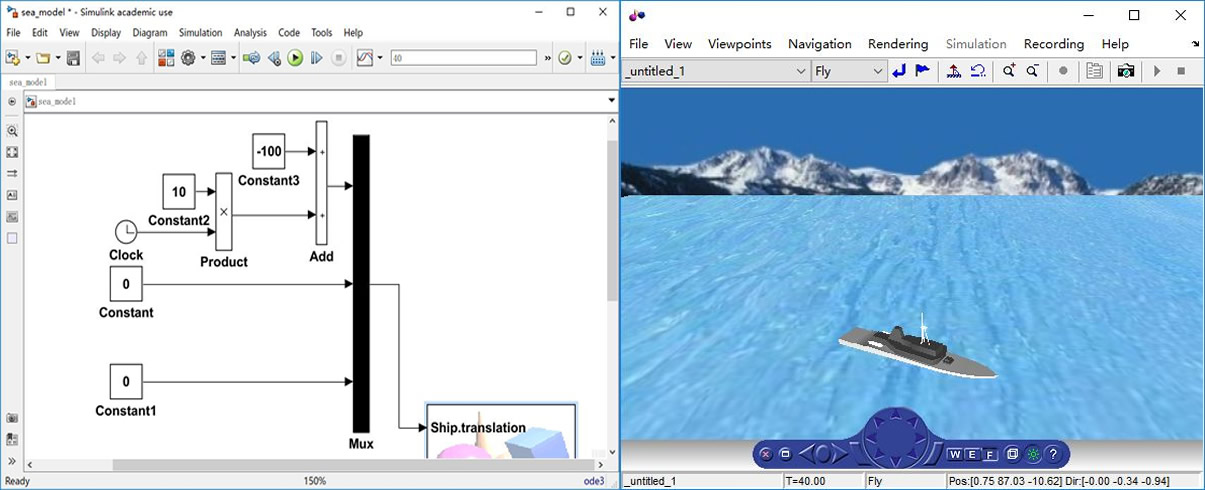
\includegraphics[scale = 0.5]{image/simu3dan.jpg}
  \caption{A sailboat simulation with simulink 3d Animation}
  \label{fig:simu3dan}
\end{figure}

A beginner can do a visualization of real-time simulations after tens of minutes study. That is an advantage if we just have not much time to simulate, especially it is on 3D.\\

\subsection{How does it work ?}

It works by providing applications to link Simulink and MATLAB algorithms to 3D graphics objects. It allows us to view and check the dynamic behavior of the system in a virtual reality environment. The objects are represented in Virtual Reality Modeling Language (VRML), a standard 3D modeling language. We can animate a 3D world by changing its position, rotation, scale, and other object properties during desktop or real-time simulation. We can also inject virtual sensor signals and access the 3D animation data in Simulink or MATLAB for post-processing. Simulink 3D Animation includes viewers for rendering and interaction with virtual scenes. With 3D World Editor, we can create detailed scenes assembled from 3D models exported from CAD or web-based sources. We can incorporate multiple 3D scene views into the MATLAB figures and interact with these views by a hardware device as simple as a mouse.

\section{Matplotlib}

\subsection{Presentation}
\footnote{Section written by N.Mehdi } 
Matplotlib, created by John Hunter (1968-2012), is a Python 2D plotting library composed of several toolkits like 3D plotting, real-time plotting, mapping toolkits and more. With NumPy, Python provides an object oriented API for data programming and scientific visualizations sharing some features with MATLAB.

\subsection{Operating Structure and Code Elements}

Displaying a simple looking animation with matplotlib was the easier way to obtain an animated representation of the simulation running under ROS. To do so, we had to just create a ROS package dedicated to plotting a 2D simulation. It was one of the strengths to use Python and the associated libraries. Everything is running under the ROS ecosystem and we do not need to export the data from the simulation toward an external program. We access the data through regular subscribers.
For more details on how the different ROS packages including the Python display, we could refer to the Chapter 4 Section 4.2. 

\begin{figure}[H]
  \centering
  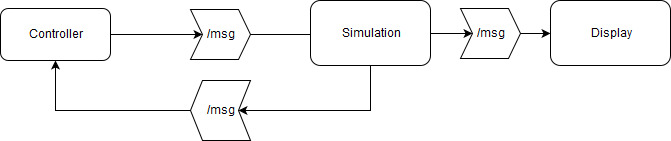
\includegraphics[scale = 0.6]{image/index.jpg}
  \label{Flow}
  \caption{Messages flow between the simulation and the display }
\end{figure}

\subsubsection{Code Structure}

The whole code used for the Matplotlib display is inside the dedicated ROS package. Each element, from the sailboats to the buoys, is represented by an instance of the \textit{PoseHolder} class which is the mother-class of \textit{SailboatPoseHolder} and \textit{BuoyPoseHolder}. This family of classes contains the objects which will be influenced by the environment like the wind direction and regulated by the controller. For the sailboat, the parameters are x, y and $\theta$ while the buoy location is represented by x, y and z. Each object has a parameter history for each component, allowing the regulator to access to the previous locations  of the objects. 


\lstset{
    string=[s]{"}{"},
    stringstyle=\color{green},
    comment=[l]{:},
    commentstyle=\color{blue},
    keywordstyle=\bfseries\color{green!40!black}
}
\renewcommand{\lstlistingname}{Code}
\begin{lstlisting}[caption=PoseHolder Class, frame=single,language=Python]
class PoseHolder(object):
    """docstring for SailboatPoseHolder"""
    MAX_HIST_SIZE = 500

    def __init__(self, pose):
        self.pose = pose
        self.histX = []
        self.histY = []
        self.histT = []

    def update_hist(self, x, y, theta):
        self.histX.append(x)
        self.histY.append(y)
        self.histT.append(theta)
        if len(self.histX) > PoseHolder.MAX_HIST_SIZE:
            del(self.histX[0])
        if len(self.histY) > PoseHolder.MAX_HIST_SIZE:
            del(self.histY[0])
        if len(self.histT) > PoseHolder.MAX_HIST_SIZE:
            del(self.histT[0])
\end{lstlisting}

Different functions allows to update the  parameters calculated by the simulation package and read by the publisher. These update functions are called in a \textit{while} loop, animating the different objects on the display. The principal update methods are given in the following.  

\renewcommand{\lstlistingname}{Code}
\begin{lstlisting}[caption=Update Functions, frame=single,language=Python]
def update_disp(msg, name):
    global sailboats, buoys
    # print 'Updating', sailboat_name
    # print('[INFO] updating : {}'.format(name))
    if name in sailboats:
        # print('[INFO] Adding new sailboat pose : {}'.format(name))
        sailboats[name].add_new_pose(msg.pose)
    else:
        buoys[name].add_new_pose(msg)


def update_wind(msg):
    global wind_dir, wind_strength
    wind_dir, wind_strength = msg.wind_angle, msg.wind_strength


def update_center(msg, name):
    global sailboats, buoys
    # print 'Updating center', sailboat_name
    if name in sailboats:
        sailboats[name].cx = msg.data[0]
        sailboats[name].cy = msg.data[1]
    else:
        pass
\end{lstlisting}



\subsubsection{Sea Plot Utility}
A separate module called \textit{sea\_plot\_utility} was used to provide the drawing functions. Each function within gives a Numpy array (vector or matrix), which is called in the main file for each drawn objects. 
\subsection{Result}

Once the launch files executed, we have the following display. The sailboats leave a green trail behind them and the opacity of the buoys represent the depth and the black arrow gives the wind direction. 

\begin{figure}[H]
  \centering
  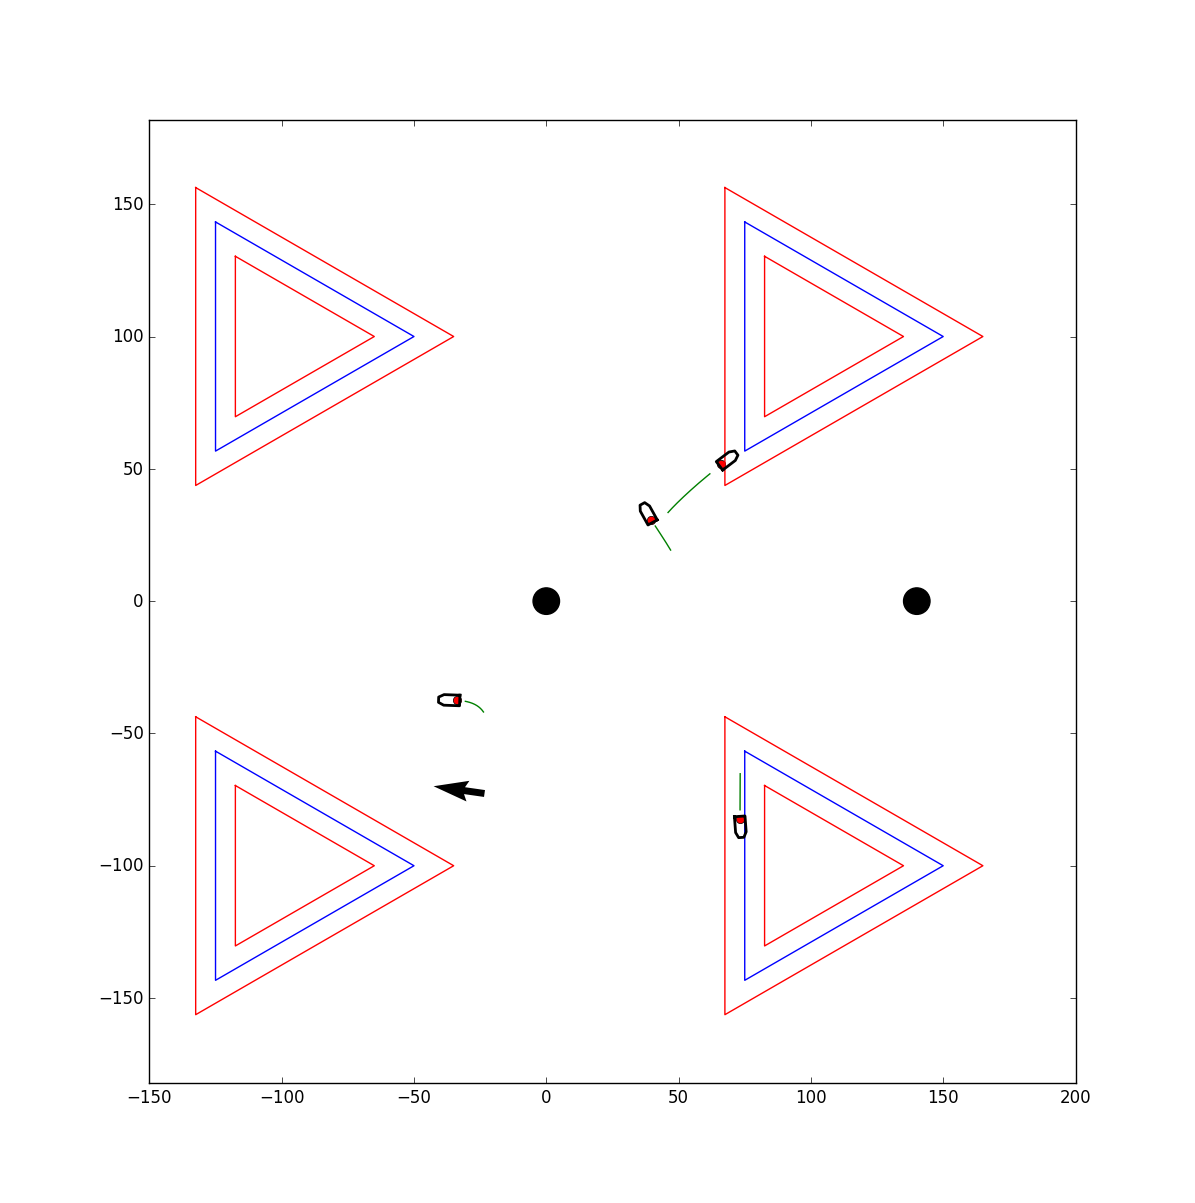
\includegraphics[scale = 0.4]{image/display3.png}
  \label{Flow}
  \caption{Display with matplotlib plotting }
\end{figure}




\section[OpenGl]{OpenGL\footnote{Section 5.2 written by Pierre BENET}}

\begin{figure}[htbp]
  \begin{minipage}[b]{0.4\textwidth}
  \centering
    
\includegraphics[scale =0.3]{image/opengl.jpeg}
  \end{minipage}
  \hfill
  \begin{minipage}[b]{0.4\textwidth}
  \centering
    
\includegraphics[scale = 0.3]{image/SDL.jpeg}
  \end{minipage}
\end{figure}

\subsection{Presentation}

Open Graphics Library (OpenGL) is a cross-language, cross-platform application programming interface (API) for rendering 2D and 3D vector graphics. The API is typically used to interact with a graphics processing unit (GPU), to achieve hardware-accelerated rendering.

We chose to use OpenGl 1.1 as a soft and reliable 3d rendering system. OpenGl is a low level rendering library. Unlike high level graphic engine such as Unity, it is easy to print vector fields and soft graphic that are easy to see. With realistic graphics, it can be difficult to see the data between the reflects of the light and the real opacity of watter for example. With Opengl, transparency of watter can be adjusted for a better visualization.

OpenGl does not work alone. It has to be integrated in the window manager of the operating system. An open source library SDL (Simple Direct media Layer) enables to use the graphic interface of most of the operating systems. Moreover, it provides keyboards and mouse support so that the user can navigate in the 3d environment and interact with the window. SDL provides also a lot of features such as sound handling and other device support.
 
\subsection{3d features}

The 3d geometric object that we print are the sea, the boats, the buoys, the vector fields, the grid pattern and the localisations of the intervals. The sea is made of two layer of transparent blue sqares, so that looking to the sea from the outside looks darker that from the inside. And everything that is in the sea looks blue. The boats geometry have been recovered from an older sailboat control simulation. The veil and rudder are movable. The buoys are simple red spheres.

% IMAGE: shepherd opengl rendering
\begin{figure}[H]
	\centering
    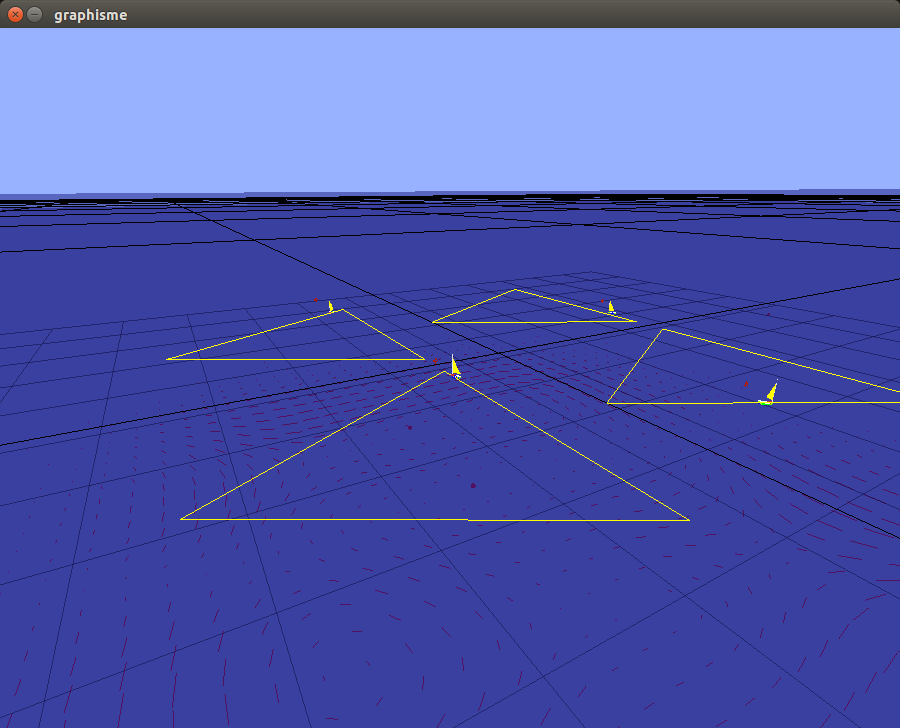
\includegraphics[scale=0.4]{image/shepherd_opengl.png}
    \caption{simulation rendering with opengl and SDL}
\end{figure}


\subsection{Camera control}

The camera control system is a first person view. The camera can be controlled in the six local axis of the view (three rotations and three translations) thanks to the mouse. This enables a practical and intuitive navigation in all directions.

The mouse wheel enables to move forward and backward. holding the left mouse button of the camera while moving the mouse moves the scene perpendicularly to the camera. holding the right mouse button while moving the mouse rotates the camera on an axis perpendicular to the camera axis. holding both right and left button enables to rotate the camera on its axis.

Camera handling is often used by an extern 3 by 3 matrix system that has to be implemented. However, this time, only the OpenGl transformation system has been used to control the camera. OpenGl possessed its own matrix 4 by 4 stack that includes rotation and translation and also includes multiplication function and generation of basic matrix such as rotation and translation matrix. The purpose of this matrix stack is to apply successive affine transformation to the geometry. But we can use it as a computationnal tool. OpenGl provides a function to store in our program the current transformation matrix. So to compute matrix multiplication and rotation matrix generation, we will store the current matrix transformation in a variable; load the matrix we want on the OpenGl matrix stack; compute transformations; get the result in an other variable; put back the initial transformation result so that OpenGl has seen nothing.

\subsection{Communication with the Simulation}

The communication between the simulation and the OpenGl rendering is a client-server link. The simulation is a server on which the OpenGl display connects. As the OpenGl display is soft and very compatible, it can be run on any distant computer, while the simulation need ROS to run.

The communication is binary, allowing a very effective communication. The client and the server know the data structures and just copy part of the communication buffer into structures. The structures are composed of the state variables of the Buoys and Sailboats.

\renewcommand{\lstlistingname}{Code}
\begin{lstlisting}[language=C++, caption={display opengl communication structures}, frame=single]
class Sailboat0
{	
    public:	
        double x,y,theta,phi;// position and orientation
	
        double fg,fv,gamma,deltav,deltag,deltavmax;  //link variables
        double a,psi;// wind            
            
        double cx,cy;// triangle center
};

class Buoy0
{
    public:
        double x;// position x
        double y;// position y
        double z;// position z
        double Xdot[3];// Buoy speed
};
\end{lstlisting}

\section{Unity3D}
% IMAGE: Logo Unity*
\begin{center}

\includegraphics[scale=0.05]{image/unity-logo.png}
\end{center}
\subsection{Presentation}
\footnote{Section written by Anthony Welte and Camille Soulié}

Unity3D is a game engine developed by Unity Technologies. It is widely used in the development of video games, especially on mobile devices and websites because it is one of the most lightweight game engine available. It uses the aforementioned OpenGL API to use the processing power of the machine it is installed on. It also provides an abstraction level allowing the programmer to easily add 3D Objects in a scene, manage lighting and shading options, textures, sound effects and many other functionalities. Unity also offers a physics engine that can compute collision, gravity as well as more complicated patterns such as moving cloth and water. 

In our project we use Unity as a graphical engine, it was decided not to use the physic engine in order to have complete control over the behaviors of the sailboats and buoys. The simulation program computes the state of the world, this is then send to Unity that displays the new state of the world. Because Unity is intended to be used more as a pleasing graphical tool than a exact representation of the simulation, liberties may have been taken on the position of the objects in order to obtain smoother movements.

Finally Unity provides powerful libraries which allow us to display a very realistic simulation. However the position of the objects on the screen depends on the frame rate which depends of the platform used to display the simulation. Therefore the display may be delayed compared to the simulation. In fact, the purpose of Unity in this project was mainly to render the simulation with a high graphic realism and this may be an additional asset to eventually convince a customer more easily. Furthermore the use of Unity3D can be extended with virtual reality since it is compatible with some VR devices such as the Oculus Rift or the HTC Vive. 

\subsection{The Environment of Simulation}
\subsubsection{Graphical Objects}
\footnote{Section written by P.Martin and Z.El Abdalaoui}
As it has been said Unity gives us a great freedom in the creation of environment even with the free version. Thanks to a large number of librairies (more precisely called assets) it is possible to create a realistic scene using water,trees,skybox,ground modeling etc.
In our project the main purpose was that Ifremer's team could recognize something like the "Rade de Brest" with its huge bridge, coasts ,Ifremer's building. On the whole, the scene has been created in 4 stages.

\begin{itemize}
\item The first step has been the creation of the ground. Unity provides a large range of tools allowing different modifications of ground's shape.So, we create our plane as a GameObject, then we can add on it several components. In order to create a wide area of sand we added a sand texture, it is just a jpg file which will be repeated many times on the plane. Like that the plane looks like a real (almost) sea floor. 
\item Now that the texture applicated, it is possible to model the terrain on our own. For this we used a very useful tool. Thanks to this feature, changing the elevation (relief) of our plane. This works like a brush. We can define it size (diameter) and the maximum altitude reached by the plane. It exists several brushes, some create peaks, others just elevated platforms. It is really interesting to model his own plane. you can spend several hours on this task if you want details. Finally here modeling yields this result:

% IMAGE: modeling plane + initial plane
\begin{figure}[H]
	\centering
    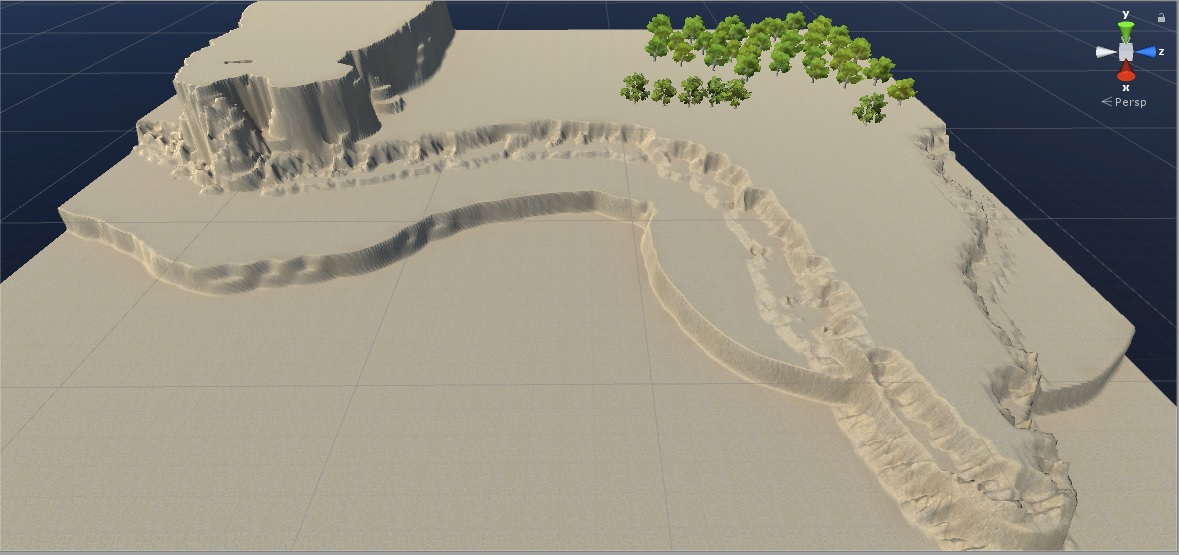
\includegraphics[scale=0.4]{image/unity2.jpg}
    \caption{Plane with texture and after modeling}
	\end{figure}
    
\item The next step consists in adding the main asset of the project. It is not exactly a long step because water plane is already a very powerful asset implemented in Unity. This one allows us to display a very realistic sea plane. We decided to put a reflective water mode. It means that only the sky is reflected on the surface and the water is not transparent too. Several water assets exist in unity, some of them are able to generate waves, movement on the water. However in this project we decided to leave these modules and just keep a simple water. A calm ocean.


\item To create a realist scene, we need environment (ground,water,sky..) but also need some 3D objects like building, bridge or road. For this part the community helped us. Indeed thanks to the online 3D library TF3D people share their creation. To display Ifremer's building we used a 3D object representing building which look like Business Office, then to remember the "Rade of Brest" we used a huge bridge.

It is possible and easy to import in Unity stl files or 3D files or Blender files. Keep in mind that we used Unity for the represention and for the graphic performances. However it is really hard to draw or model an accurate object as a boat,or a car with simple assets. (square,plane,circle..) Thus, working on Unity invited us to work on other software (which we did not master or never used at all). This was actually interesting to discover Blender and all the abilities it provides for 3D modeling,Video making, visual rendering etc.




% IMAGE: d'un objet
\begin{figure}[H]
	\centering
    \caption{Buoy (left) and Sailboat (right) models}
    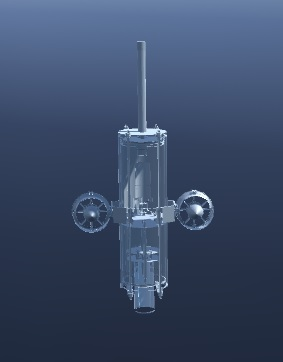
\includegraphics[scale=0.6]{image/buoy.jpg}
    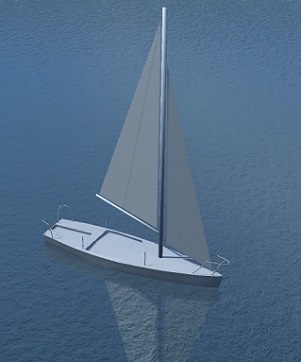
\includegraphics[scale=0.6]{image/Sailboat.jpg}
	\end{figure}
    
\item Finally, the last object to control is the camera. Indeed in Unity you can see how does your scripts or your objects behave in the scene with a Camera item. It was crutial for the project in order to observe how our boats and buoys move to drive the camera. We control our camera with the keyboard for the elevation, and the left right turns .And the rotation is controlled with the mouse. We also created a script which allow us to displace the camera as we want.
\end{itemize} 

In short, the creation of the scene is a long process because it always need some adjustements. Please find in the 5.3.5 part the final result of our scene.
We can note that even if the result is acceptable we tried to improve it. We tested on script of buoyancy in order to simulate the real boat's movement on the ocean. However that script was not easy to use , so we gave up on this way because it was really hard to control the flux of waves (back and forth). Then we could add the rotation of the sail as a function of the wind. This idea was envisaged, and was not difficult to implement, but we left it aside in order to focus on the localisation of the squad. Finally the final scene is really sufficient and the project seems greatly correspond to expectations even if Unity allows to us to improve it again and again.

\subsubsection{Buoy and Sailboat creation}
After creating the environment in which the boats and the buoys will move, we need the actual object to display in the scene
\begin{itemize}
\item As previousely mentionned, the Unity3D community shares many game objects of their own to use. We used one of these assets found online to represent the sailboats onscreen. But we had to add some more textures to create a realistic sailboat. For instance, since the textures are only seeable from one side, only one side of the sail was displayed. Then to be able to move the sail yaw, we had to split it from the original game object in order to make the sail movable around the mast.

\item The adding of the buoy was much more simple. First we tried to draw the buoy from scratch but as explained in the previous part, it is not something easy to do with the time at our disposal. But in the end we were provided with a 3D CATIA model of a buoy similar to the one usually used. Then we just had to import the model on Unity to display it.
\end{itemize}

Once the creation of the objects and the scene were done, we could link them to the client-server architecture that manage the position of all the items onscreen. (ie the position of the boats and buoys, the depth of the buoys, the sailboat, and sail yaw.)
% TODO

\subsubsection{SimulationManager}
\footnote{Section written by Anthony Welte and Camille Soulié}
SimulationManager is the main object of the scene. It has two scripts TCPServer.cs and SimulationManager.cs that provide communication with the simulation and dynamically instanciate the objects (sailboats and buoys). 

TCPServer.cs is the implementation of the client-server architecture. It listens to the simulation and records a stream of one or several JSON strings. This stream is then processed to extract individual JSON string that are then sent to SimulationManager.cs.

SimulationManager.cs extracts the data of the messages received from TCPServer.cs and stores them in a queue. Then at every new frame displayed, SimulationManager dequeues a message (if there is one) and updates the scene. It either creates a new object if the message corresponds to a new object or updates the state of an existing entity. 
We have tried to interpolate the position of the different entities between two received positions in order to reduce the number of messages sent by the simulation but this was more complicated than predicted and this functionality is not fully operational yet. That is why we have chosen for now to increase as much as possible the data flow between the server and the client in order to have the most fluid display possible. % TODO

\subsection{Communication with the simulation}
\subsubsection{Server-Client link}
\footnote{Section written by Anthony Welte}

To communicate between the simulation and Unity, a client-server architecture has been chosen. This choice has several advantages:
\begin{itemize}
\item A modular architecture: enabling the two programs to work independently and making the development of the programs easier to split into two separate teams.
\item An online architecture: enabling the programs to run on a same machine or on distant machines
\item A language agnostic architecture: enabling the simulation and the display to use different languages (C++ for the simulation, C\# for Unity)
\end{itemize}

\subsubsection{JSON format}
\footnote{Section written by Anthony Welte}
To communicate data, JSON parsing is used. This method format variables (test, numbers, etc) into a text that contains all the variables and that can be easily extracted by Unity. JSON was introduced by Javascript but libraries are know available on most mainstream languages making it an ideal solution to communicate data between two languages

\lstset{
    string=[s]{"}{"},
    stringstyle=\color{blue},
    comment=[l]{:},
    commentstyle=\color{black},
}
\renewcommand{\lstlistingname}{Code}
\begin{lstlisting}[caption=JSON format, frame=single]
{
    "Sailboat":
    {
        "name":"Auv0",
        "sailYaw":-13.1802,
        "x":-19.2049,
        "y":20.338,
        "yaw":-296.908
    }
}
\end{lstlisting}

This formating made it easy to add a the buoys later in the project. % TODO

\subsection{Results}
\footnote{Section written by Camille Soulié}
Since the aim of this part of the project is to display a scene, the results of our work is better described by images than by words. You can see below a screenshot of a scene displayed with Unity that gives an good overview of what have been done. We can notice the high realism of the display. Unity can indeed handle the shadows, the reflects, the ripples on the water...

\begin{figure}[H]
	\centering
    \caption{Screenshot of a scene displayed with Unity3D}
    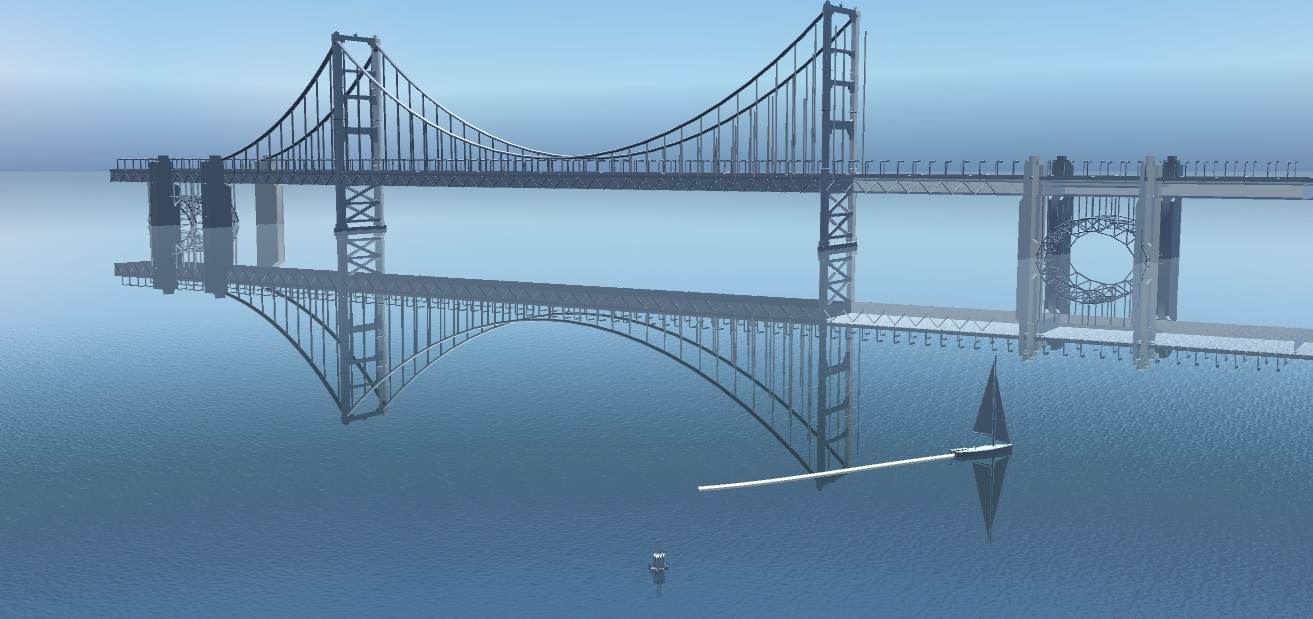
\includegraphics[scale=0.5]{image/DisplayUnityResult.jpg}
	\end{figure}
% IMAGE
\subsection{Thought for enhancement}
\footnote{Section written by Camille Soulié}
As mentioned earlier, one way to optimize the display of the simulation might consist in in interpolating the position of the entities between two successive positions and therefore in drastically reducing the data flow between the client and the server. That will enable both more fluidity and the workload decrease of unity.
We can also add some textures on the entities or some atmosphere sounds like seagull calls, sail slams, slappings... to increase the realism.

% ===================== Conclusion ====================
\newpage

	\begin{center}
		\textbf{\LARGE{Conclusion}}
	\end{center}

\vspace{5cm}

\footnote{Section written by M. Fadil Ennouhi and L. Zhu, reviewed by Simon Chanu}
In this project, we constructed a mathematical model as well as a simulation with visual display. At the very beginning, all the theoretical basic concerned are reviewed. We have used the method of interval analysis and TDOA, by which we built the basic equations. Next, we did several studies on the tools for better work condition and parfait group cooperation. Tools like GitHub and scrum bring us more efficiency . We worked as a group rather than only work separately on each party. Furthermore, we constructed the architecture to solve the simulation problem and let it be optimized. We have used ROS(Robot Operating System) as the kernel instrument. We simulated the environment, the boat and the buoys under ROS. At last we did some visual model on 2D and 3D platform. This allow us to explain the simulation to the public. The production of this experiment is quite useful in further researches.\\

Despite of the ambitious nature of the SHEPHERD project, we remain confident of its feasibility. All the assumptions made in our working simulation remain compatible with the real world environment. We demonstrated in this report a working simulated prototype relying solely on existing techniques and sensors.\\

As mentioned, the Robot Operating System coupled with GitHub enabled our relatively large team to work independently in small groups and each group handled a specific module of the project without risking the compatibility of the pieces. Perhaps the most noteworthy example of this seamless integration is the Unity video rendering which allows the viewer to quickly grasp the functioning and the purpose of the project while remaining faithful to the algorithms and physics of the project.\\

We got a great deal of progress from working on this project. In the three months of activity, first of all, the most direct acquisition is on the professional techniques. We did not only practice the knowledge acquired in class, such as interval analysis, but also made ourselves more skilled by learning numerous new skills. We had 17 different mini courses in a variety of subjects. And each one gave us an opportunity to optimize our processes of work. In addition, we worked three months in a cooperative environment. Working as a team is not easy as imagined but we achieved this successfully. Solidarity and cooperation are the fruit for the effort we had payed.  Last but not the least, we experienced what a real project looks like. It is more close to a professional job, thus making us better and faster at adapting to a working life and rhythm after graduation.

\newpage
%récupérer les citation avec "/footnotemark"
\nocite{*}

% ====================== Biblio ======================

%choix du style de la biblio
%\bibliographystyle{plain}
%inclusion de la biblio
%\bibliography{Rapport2A}
%voir wiki pour plus d'information sur la syntaxe des entrées d'une bibliographie


% ====================== Annexes ======================
\newpage

	\begin{center}
		\title{ \HRule{} \\ [12cm]
				\LARGE \textbf{\uppercase{Annexes}}\\ [12cm]
				\HRule{}}
		\maketitle
	\end{center}

\end{document}
